\documentclass[12pt,a4paper]{article}

\usepackage{setspace}
\onehalfspacing
\usepackage{caption}
\usepackage{subcaption}
\usepackage{float}
\captionsetup[table]{font={stretch=1.5}}     %% change 1.5 as you like
\captionsetup[figure]{font=onehalfspacing}    %% change onehalfspacing as you like
\usepackage[english]{babel}
\usepackage[utf8]{inputenc}
\usepackage{amsmath}
\usepackage{amssymb}
\usepackage{graphicx}
\usepackage[colorinlistoftodos]{todonotes}
\usepackage[top=0.75in,left=0.75in,right=0.75in,bottom=0.75in]{geometry}
\usepackage{multicol,caption}
\usepackage{makeidx}
\usepackage{pdfpages}
\usepackage[compat=1.0.0]{tikz-feynman}
\usepackage{hyperref}
%\usepackage{LuaLaTeX}
\makeindex
%\usepackage{fixltx2e}
\usepackage{cite}
\newenvironment{Figure}
  {\par\medskip\noindent\minipage{\linewidth}}
  {\endminipage\par\medskip}
\setlength{\columnsep}{1cm}
\setlength{\parindent}{0pt}
\usepackage{color,soul}
\usepackage{booktabs}
\newcommand{\ra}[1]{\renewcommand{\arraystretch}{#1}}

\title{Analyzing the response of the VIDARR detector\\
	\large PhD Thesis\\~\\}
\date{\today}
\author{Ronald Collins ID:200948843}

\begin{document}
\maketitle

\begin{Figure}
 \centering
 
\includegraphics[width=1.0\linewidth]{Liverpool_logo}
 \captionof*{figure}{} 
\end{Figure}


\begin{center}
\textit{Department of Physics, High Energy Physics\\}
\textit{VIDARR collaboration\\}
\end{center}


\pagenumbering{gobble}
\newpage
\pagenumbering{roman}
\begin{abstract}
\normalsize Understanding the physical response of the Verification Instrument for Direct Assay of Reactors at Range (VIDARR) detector through Monte Carlo simulation allows for signal and energy discrimination. It allows for modelling with no noise, each particle's energy is known and can be reconstructed allowing for simulated efficiency calculations. It is possible to determine energy losses at several stages such as deposition, escaping events and attenuation as well as energy lost through hard scattering off of the TiO$_2$ coating on a single bar.  Reconstructed energy is then smeared through Poisson statistics to approximate measured quantised data. Using this simulation a simulated trigger is constructed with $\sim$ 70\,\% neutron efficiency. This Monte Carlo simulations is parallelised allowing for efficient implementation of high performance computing (HPC), generating large statistics. This leads to an anti-neutrino detector efficiency of $\sim$ 69\,\% for the original detector (1862 bars) and $\sim$ 78\,\% for the upgraded detector (2660 bars).\\
\providecommand{\keywords}[1]{\textbf{\textit{Keywords:}} #1} %Keywords command has to be supplied manually
\keywords{Monte Carlo, Geant4, High performance computing (HPC), Anti-neutrino}
\end{abstract}
\vspace{5mm} %5mm vertical space before main body of text
%\begin{multicols}{2}
\tableofcontents
\newpage

\pagenumbering{arabic}
\section{Introduction (Literature Survey)}
\subsection{VIDARR's Aims}
The Verification Instrument for Direct Assay of Reactors at Range (VIDARR) is a plastic scintillating detector that aims to measure reactor activity for non-proliferation and potential waste burn up. Reactor activity will be determined through the measurement of anti-neutrinos and their corresponding energies. Reactor activity will be measured through the process of inverse $\beta$ decay (equation \ref{inverse_beta_decay}). Further, the VIDARR project aims to deliver this in a portable and standard form factor that can be deployed outside the security cordon of a standard power generating reactor ($\sim$ 60\,m). The simulated responses of the upgraded VIDARR (2660 bars) detector will be the focus of this report, with comparisons to the original (1862 bars) detector being included for comparison. All plots in this report referring to VIDARR are simulation-based.

\subsection{Anti-neutrino reactor monitoring}
Nuclear reactors produce high quantities of anti-neutrinos ($10^{20}$ per GW$^{Th}$ of power \cite{muller_reactors}). Anti-neutrinos are produced in fission chains within reactors via beta decay, shown in equation \ref{beta_decay} where a neutron decays to a proton giving off an electron and electron anti-neutrino.
\begin{equation}
n \rightarrow p + e + \overline{\nu_{e}}
\label{beta_decay}
\end{equation}
The electron anti-neutrinos that are produced by the reactor are useful as they cannot be shielded due to their small cross section of the order 10$^{-42}$\,cm$^2$\cite{vogel_beacom_nu_cross}. In 1978 \cite{an_proposed} the idea of electron anti-neutrino detection from reactors for accounting the fissile inventory was proposed. The mechanism for this process is inverse $\beta$ decay, which is shown in equation \ref{inverse_beta_decay}, where an electron anti-neutrino interacts with a proton giving off a positron and a neutron. This gives a double coincident signal, with the prompt component from the positron and the delayed (by O $\sim$ 10 $\mu$s) from the neutron, this distinct signature allows for detection of the event.
\begin{equation}
p + \overline{\nu_{e}} \rightarrow n + e^+ 
\label{inverse_beta_decay}
\end{equation}

Recently, interest in non-proliferation has increased and become a more important issue, this increasing interest led to a first demonstration in 2007  \cite{songs_s1}, which detected anti-neutrinos from two reactors installed in San Onofre Nuclear Generating Station (SONGS). However, this prototype (SONGS1) had two major drawbacks: it used vacuum photon multiplier tubes, which are expensive and fragile, and used liquid scintillator. Liquid scintillator is relatively inexpensive, so high mass detectors are easier to build which is necessary when looking for small cross section particles, but is a biological and fire-hazard. In 2008 \cite{IAEA_bio_fire_report} it was suggested that hazardous liquids should not be used in future, due to safety concerns. The SONGS1 prototype also had the advantage of being below ground (providing \approx 25\,m of water equivalent overburden\cite{songs_s1}) and inside the reactor building, shielding it from cosmic rays and other sources of background radiation. However, for a prolonged operation of reactor monitoring being positioned inside the reactor building poses increased safety risks, and is difficult to access (for example for retrofitting), and so is deemed undesirable by plant operators. 


%Need to do a section on how VIDARR works, I need to find the 

\subsection{Existing Reactor monitoring programs}
Since SONGS1 there have been multiple reactor anti-neutrino monitoring experiments. Below in this subsection two different alternate reactor monitoring programs (PANDA and SoLid), and a baseline measurement based at a nuclear facility (Double Chooz) are discussed. The methods of execution vary from the VIDARR detector and each other. 
\subsubsection{PANDA}
The Plastic Anti-Neutrino Detector Array (PANDA) is a segmented detector that uses plastic and Gadolinium shown in figure \ref{sub_pana_close}, the gadolinium's interaction with neutrons is shown in equation \ref{Gd_eq}. The bars clustered together can be seen in figure \ref{sub_panda_far}. The bars seen in figure \ref{sub_panda_far} are plastic scintillator with dimensions of 10\,cm $\times$ 10\,cm $\times$ 100\,cm with two 10\,cm\ $\times$ 10\,cm $\times$ 10\,cm acrylic cubic light guides are glued to both ends of the plastic scintillator with optical cement capped with photon multiplier tubes at either end of the bars for data collection \cite{PANDA_2014}. The interior of a plastic scintillating bar can be seen in figure \ref{sub_pana_close} which also shows the prompt and delayed event of an $\overline{\nu_e}$ event. In addition calibrations and comparison to Geant 4 \cite{geant4_ref} have been performed with a baseline of a $^{60}$Co with reasonable agreement between the calibration source and the simulated response \cite{PANDA_2012}. 

\begin{equation}
n + {^{155,157}Gd} \rightarrow {^{156,158} Gd} + \gamma (\sim 8\,MeV)
\label{Gd_eq}
\end{equation}

\begin{figure}[H]
\centering
\begin{subfigure}{.5\textwidth}
  \centering
  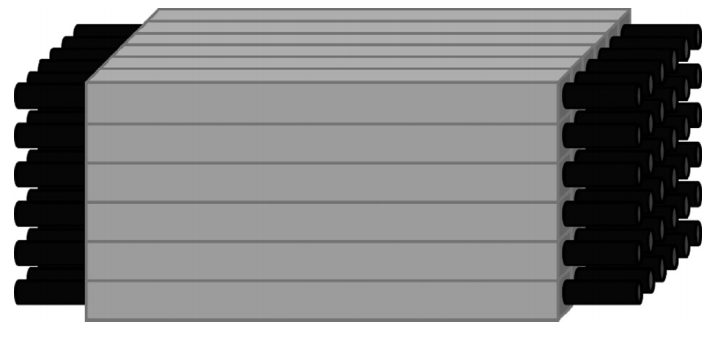
\includegraphics[width=\linewidth]{panda_far.png}
  \captionsetup{width=.9\linewidth}
  \caption{Exterior of PANDA bars are clustered together with photon multiplier tubes at the end to measure photons, from \cite{PANDA_2014}.}
  \label{sub_panda_far}
\end{subfigure}%
\begin{subfigure}{.5\textwidth}
  \centering
  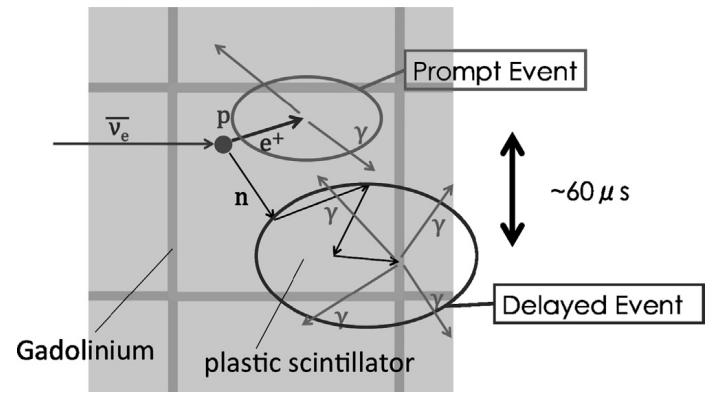
\includegraphics[width=\linewidth]{panda_close.png}
  \captionsetup{width=.9\linewidth}
  \caption{Interior of the PANDA detector, prompt event of a positron and delayed gadolinium capture and cascade from a neutron event, from \cite{PANDA_2014}.}
  \label{sub_pana_close}
\end{subfigure}
\caption{Exterior (\ref{sub_panda_far}) and interior (\ref{sub_pana_close}) of the PANDA detector.}
\label{pana_close_and_far}
\end{figure}

The bars are not positioned perpendicularly in the $z$ direction (figure \ref{sub_panda_far}). Therefore tracking is more difficult in PANDA, due to not having specific $x$ and $y$ coordinates, this makes vetoing cosmic muons (a major source of background) potentially harder in PANDA than if the bars were perpendicular. The photon multiplier tubes (PMTs) used in PANDA are also expensive, the PANDA36 shown in figure \ref{sub_panda_far} is much smaller than the proposed final design of 100 channels and 1m$^3$ \cite{PANDA_2012} but PANDA is being built in stages because of the expense of these components. However, the potential for measuring many photons with high efficiency makes PMTs attractive. Both Lesser PANDA (16 channels) and PANDA36 have been deployed by van with background measurements and reactor measurements being taken from inside the van \cite{PANDA_2012}, \cite{PANDA_2014}. But due to the flammable nature of petrol and diesel it is unclear weather reactor operators would be open to having a van stationed indefinitely outside their reactor buildings. PANADA36 has also been used for monitoring Terrestrial Gamma-ray Flashes (TGFs) from thunderstorms to allow for further background reduction at nuclear sites\cite{PANDA_tgf}. 

\subsubsection{SoLid}
The SoLid detector is a plastic scintillating detector that uses wavelength shifting (WLS) fibres with MPPCs at the end to read out fibre signals and adjacent 5\,cm $\times$ 5\,cm $\times$ 5\,cm cubes being lit up at similar time intervals to discern particles \cite{Solid_proposal}. There is a prompt signal outputted from the positron in the plastic cubes and a delayed signal from the $^6$LiF:ZnS(Ag) screen interacting with neutrons as shown in figure \ref{Solid_cub_diagram}. The prompt positron response and delayed neutron response is similar to PANDA and Double Chooz. In SoLid $^6$Li is used as the neutron capture agent (equation \ref{Li_interact_eq}), as opposed to Gd used in PANDA and Double Chooz (equation \ref{Gd_eq}), produces an $\alpha$ and a 4.78\,MeV $\gamma$ \cite{Solid_readout}. The $\gamma$ signal is ignored because the $\alpha$ signal produced is clear and produces a specific pulse shape signal \cite{Solid_readout} which has very minimal background due to its specific pulse shape. 

\begin{equation}
n + {^6Li} \rightarrow {^3H} + \alpha +4.78\,MeV
\label{Li_interact_eq}
\end{equation}

\begin{Figure}
 \centering
 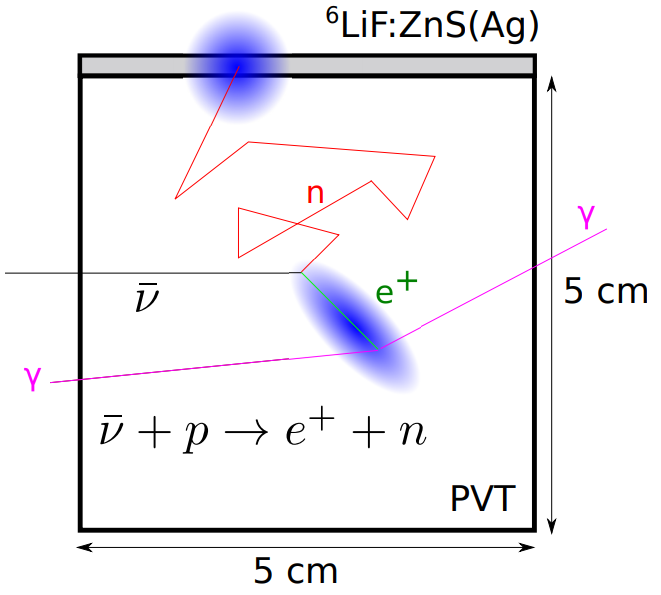
\includegraphics[height=58mm]{SoLid_cube.png}
 \captionof{figure}{SoLid cube during an inverse beta decay event anti-neutrino decays into a positron and neutron via equation \ref{inverse_beta_decay}, delayed neutron is captured by $^6$LiF:ZnS(Ag) screen, positron gives prompt response from \cite{Solid_readout}.\\} 
 \label{Solid_cub_diagram}
\end{Figure}

The challenge with using $^6$Li as a neutron capture agent is producing enough light for pulse shape discrimination (PSD) to be used as analysis. The $\alpha$s need to be captured by the sulphur in the $^6$LiF:ZnS(Ag) screen which then emits a specific $\gamma$ into the plastic which in turn produces electrons via Compton scattering which are then captured by WLS fibres. The Wavelength shifting fibres may not capture enough photons for the pulse shape analysis to be used, an alternative method to this is that proposed by CHANDLER (Carbon Hydrogen Anti-Neutrino Detector with a Lithium Enhanced Raghavan-optical-lattice) \cite{aap2015}. Which uses PMT's and a Raghavan-optical-lattice to counter-act the low light issues in SoLid. However the CHANDLER design also brings challenges as the detector cannot be too large otherwise attenuation and containment of events prevents signals from being read. 

\subsubsection{Double Chooz}
The Double Chooz experiment is not a reactor monitoring experiment, instead its focus is constraining the $\theta_{13}$ measurement by measuring anti-neutrinos through inverse beta decay (equation 2). The Double Chooz experiment uses the Chooz nuclear reactors as $\overline{\nu_e}$ sources \cite{DoubleChooz06}. It's goal in 2006 was to measure the mixing angle of $\theta_{13}$ by using a far and near detector. It uses a organic liquid scintillator doped with a concentration of 0.1\,\% Gd for neutron capture. In 2012 they reported a $\overline{\nu_{e}}$ disappearance from Chooz reactors \cite{DoubleChooz_ve_disapear} stating that the data was inconsistent with no oscillations to with 99.8\,\% CL (2.9$\sigma$). This was done at a distance of 1000--1100\,m away from the reactors at Chooz for the far site and 250--300\,m for the near site \cite{DoubleChooz06}. Both sites used 10.3 cubic meters of liquid scintillator in each of the far and near detectors. As of 2015 the measurement of the mixing angle $\theta_{13}$  was $\sin^2 2 \theta_{13} = 0.090^{+0.034}_{−0.035}$, with $\sigma(\sin^2 2 \theta_{13}) = 0.015$ \cite{Double_Chooz_update}. \\\\
The detectors are situated $\sim$ 45\,m underground from the reactors as seen in figure \ref{DeepChooz} \cite{DoubleChooz06}, this makes the Double Chooz approach unsuitable for portable above ground deployment. Further the use of liquid scintillator goes against the IAEA's recommendations due to potential fire risk \cite{IAEA_bio_fire_report}. The use of dual detector sites and large amounts of scintillator has allowed Double Chooz to make detailed measurements \cite{DoubleChooz_ve_disapear} but this approach is extremely expensive and not portable. This is to be expected as the Double Chooz experiment measures neutrino oscillations, a more comparable experiment would be Daya Bay which also measures the mixing angle $\theta_{13}$ and the $\overline{\nu_e}$ disappearance. Daya Bay is significantly larger (20 tons) and also uses liquid scintillator with 0.1\,\% $^{Nat}$Gd doping. Their measurement for the mixing angle in 2017 was $\sin^2 2\theta_{13} = 0.0841 \pm 0.0027$(stat)  $\pm$ 0.0019(syst) which agrees with the Double Chooz measurement \cite{daya_bay_2017}.

\begin{Figure}
 \centering
 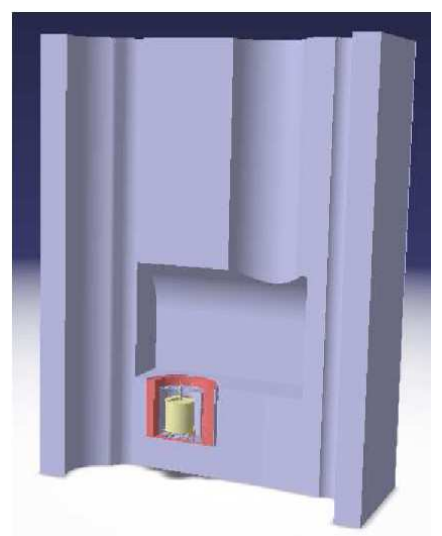
\includegraphics[height=58mm]{doubleC_deep.png}
 \captionof{figure}{The Double Chooz near site, 45\,m underground, at 250--300\, from the nuclear cores with 30\,m of overburden \cite{DoubleChooz06}.} 
 \label{DeepChooz}
\end{Figure}

\section{The Anti-Neutrino Interaction} %not really sure about the title 
The VIDARR detector observes $\overline{\nu_e}$s via inverse $\beta$ decay (equation {\ref{inverse_beta_decay}}) via the weak interaction. The weak interaction doesn't conserve flavour as inverse $\beta$ decay seen in figure \ref{inverse_beta_diagram} relies on an up quark transitioning to a down quark (uud $\rightarrow$ udd), this process can only be enabled through the weak interaction. This process is mediated through the W boson, not the, Z as the interaction has charged particles and charge must still be conserved in weak interactions. Due to the charge and colourless nature of neutrinos they only interact with other matter through the weak interaction. This leads to a small cross section of 10$^{-42}$\,cm$^2$\cite{vogel_beacom_nu_cross}, making anti-neutrinos difficult to detect. This also provides the ability for neutrinos to be observed even with significant shielding around the source. \\

In a reactor $\sim$ 200\,MeV is released per fission and 6 neutrinos along the $\beta$ decay chain are produced. ``Since unstable fission products are neutron-rich nuclei all $\beta$ decays are of $\beta^-$ type and the neutrino flux is actually pure electronic anti-neutrinos ($\overline{\nu_e}$)''\cite{muller_reactors}, meaning that the $\overline{\nu_e}$s are the main particles of interest for reactor studies. If the $e^+$ energy can be accurately measured then it would also be possible to measure the $\overline{\nu_e}$ energy as well via equation \ref{nu_energy_eq}:
\begin{equation}
 E_{\overline{\nu_e}} = E_{e^+} + (M_n - M_p) 
\label{nu_energy_eq}
\end{equation}
Which shows the $\overline{\nu_e}$ energy in terms of well known quantities, the energy of the $e^+$ and the masses of the neutron and proton \cite{vogel_beacom_nu_cross}. 

\begin{Figure}
 \centering
 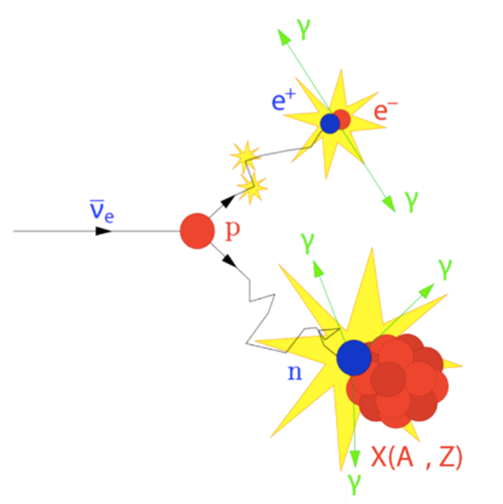
\includegraphics[height=58mm]{inverse_beta_diagram.png}
 \captionof{figure}{Inverse beta decay as the $\overline{\nu_e}$ interacts with a proton producing an $e^+$ producing a prompt response and a neutron which is capture by a nucleus.} 
 \label{inverse_beta_diagram}
\end{Figure}
% \begin{figure}[H]
% \centering
% \begin{subfigure}{.5\textwidth}
%   \centering
%    \feynmandiagram[vertical'=a to b, baseline=(a)]{
%         i1 [particle=$e^-$]
%             -- [fermion] a [dot]
%             -- [anti fermion] f1 [particle=${\overline{\nu_{e}}}$],
%         a -- [boson, edge label'=$W$] b [dot],
%         i2 [particle=d]
%             -- [fermion] b
%             -- [fermion] f2 [particle=u]
%           %b -- [fermion, half left] i2, % this produces the curved fermion line
%           %b -- [fermion, half right] i2, % this produces the curved fermion line
%     };
%   \captionsetup{width=.9\linewidth}
%   \caption{Feynman diagram for the Weak interaction of beta decay.}
%   \label{beta_decay_feyn}
% \end{subfigure}%
% \begin{subfigure}{.5\textwidth}
%   \centering
%   \feynmandiagram[vertical'=a to b, baseline=(a)]{
%         i1 [particle=${\overline{\nu_{e}}}$]
%             -- [anti fermion] a [dot]
%             -- [anti fermion] f1 [particle=$e^+$],
%         a -- [boson, edge label'=$W$] b [dot],
%         i2 [particle=u]
%             -- [fermion] b
%             -- [fermion] f2 [particle=d]
%           %b -- [fermion, half left] i2, % this produces the curved fermion line
%           %b -- [fermion, half right] i2, % this produces the curved fermion line
%     };
%   \captionsetup{width=.9\linewidth}
%   \caption{Feynman diagram for the Weak interaction of inverse beta decay.}
%   \label{inverse_beta_decay_feyn}
% \end{subfigure}
% \caption{The Feynman diagrams for beta and inverse beta deacy}
% \label{beta_and_inverse_beta_fyn}
% \end{figure}

\section{The VIDARR Detector}
The VIDARR detector is a cuboid measuring 1.52\,m wide \times 1.52\,m deep being 0.50\,m tall in the original detector be 0.70\,m tall in the upgrade (0.924\,m$^3$ volume in original to 1.62\,m$^3$ in upgraded). The VIDARR detector consists of overlapping scintillating bars with dimensions of 1.52\,m \times 0.04\,m \times 0.01\,m that are perpendicular in the $z$ axis from one another, as particles cross one layer of scintillating bars to another their position can be determined for the bars they hit. The VIDARR detector will respond to an anti-neutrino event with 1-2 bars being promptly hit by an $e^+$ and 4-5 bars being hit by a delayed (O $\sim$ $10^{-5}$\,s) neutron event. These hits emit photons which scatter through the plastic scintillator until interacting with the wavelength shifting (WLS) fibres seen in figure \ref{VIDARR_diagram} which are read by MPPCs (multi-pixel photon counters).  

\begin{Figure}
 \centering
 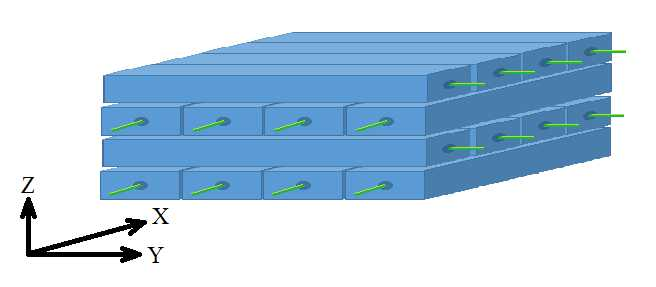
\includegraphics[height=58mm]{VIDARR_diagram.jpeg}
 \captionof{figure}{A cross section of the scintillating bars and wavelength shifting fibres of the VIDARR detector. In full detector there are 38 bars alternating in $x$ and $y$ (as shown) with 49 layers in $z$ in original and 70 in the upgraded, from \cite{gholt}.\\} 
 \label{VIDARR_diagram}
\end{Figure}
The VIDARR detector is based on a component of the T2K ND280 detector, the ND280 detector consisted of several electromagnetic calorimeters (ECals), a solenoid coil and a Magnet Yoke, which can be seen in figure \ref{ND280_det}. The term ECal applied to several different components in the ND280 detector, the downstream ECal refers to both the Barrel ECal and the P0D ECal. The original VIDARR detector was based on the barrel ECal, the dimensions of the scintillating bars (1520\,mm long by 40\,mm wide and 10\,mm deep \cite{t2k_ecal}) have not changed from T2K to the original (1862 barred) VIDARR detector to the upgraded (2660 barred) VIDARR detector. The plastic bars are therefore made from polystyrene \cite{t2k_ecal} as opposed to PVT in SoLid which would give higher light yield. However as VIDARR measures the $\gamma$ cascade from the Gd (as done in PANDA and Double Chooz) pulse shape analysis is not used so the high light yield of PVT is not required.\\\\
Changes to the overall ND280 Barrel ECal design included the removal of the lead sheets in between layers \cite{t2k_ecal}, which were replaced with Gadolinium sheets in the original and upgraded VIDARR detector. This was to include neutron capture as part of the detector's functionality so that anti-neutrinos could be accurately detected via inverse $\beta$ decay (equation \ref{inverse_beta_decay}). A cosmic muon veto was added, enabling the VIDARR detector operate above ground, which the ND280 detector did not, as underground shielding goes against the IAEA recommendations. 
%talk about the electronic briefly and then talk about the actual detector itself, the dimensions and the improvements being made to it. also potentially talk about the plastic and its properties as a scintillating medium, Ron

\begin{Figure}
 \centering
 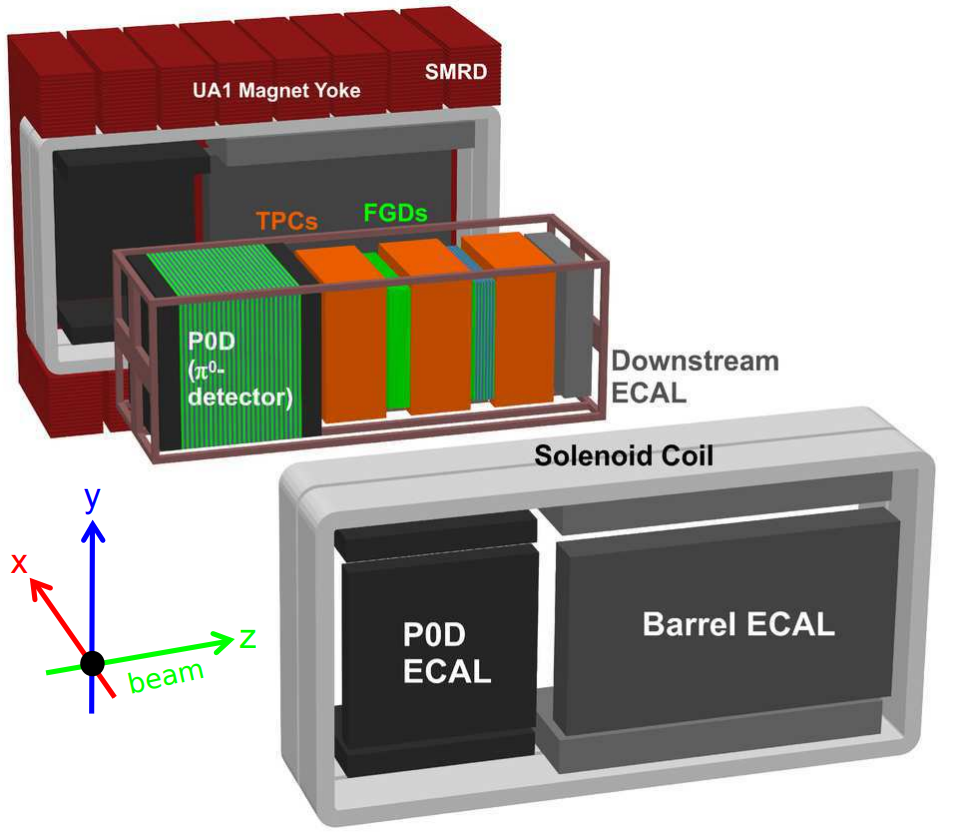
\includegraphics[height=71mm]{ND280_detector.png}
 \captionof{figure}{The ND280 detector containing the barrel ECal which VIDARR was based on, from \cite{t2k_ecal}.\\} 
 \label{ND280_det}
\end{Figure}

The VIDARR detector uses the same (WLS) fibres as the ND280 barrel ECal. The 1862 barred original detector used the multi-pixel photon counters (MPPCs) \cite{MPPC_t2k} from the ND280 detector's barrel ECal \cite{t2k_ecal} as well as the many of the other electronics. As can be seen in figure \ref{ND280_det} the set-up of the ND280 detector was designed around a neutrino beam, this means that the data acquisition  techniques that were adapted from the ND280 detector have a higher signal to noise ratio when used for a constantly monitoring detector. The trigger on the original (1862 bars) detector was a beam trigger and was therefore a forward facing trigger (in time) that had to be reversed and used integration cycles with high amounts of dead time. The upgraded  VIDARR detector will use new MPPCs and improved data acquisition techniques in order to reduce the signal to noise ratio and will be able to take data continuously with significant dead time reduction. 

%\section{Test section}

\section{Geant4 simulations}
\subsection{Single Bar Simulation}
A bar in the VIDARR detector is a plastic scintillating block it consists of the following components: A multiclad WLS fibre (split into sub components: a WLS fibre core, a fibre inner and outer cladding, a fibre mirror), a scintillating core, a multi photon pixel channel (MPPC) and coating of TiO$_2$. The level of simulation at present does not model the electronics, so the MPPC is currently a place-holder which only consists of the materials used to create the MPPC with no simulation of their electronics and so just registers all photons that interact with it.  
\\\\The single bar simulation is has a full optical model of a single bar, this is because a detailed model of the optics is needed for the production of a photon function. The simulation for a single bar is therefore more computationally intense for a single event than the full detector simulation. Modelling muons was primarily the purpose of the single bar simulation in this report. This is because they are a common source of background, understanding how they interact in our detector allows for better removal of those events. It is also easy to collect physical data as no reactor is necessary and the events are highly frequent allowing them to be used as calibration sources.\\\\
Muons are effective calibration particles due to their properties as minimally ionising particles (MIPs) \cite{pdg_passage}. In radiation passage through materials a particle is minimally ionising when it's De Broglie wavelength ($\lambda_{DB}$) is small enough to pass through matter but not energetic enough to begin showering. Assuming a density of $\sim$ 1\,g\,cm$^{-3}$ for plastic, according to the Bethe Block distribution \cite{pdg_passage}, we would expect a dE/dx of $\sim$ 2\,MeV\,cm$^{-1}$ for muons passing through carbon at $\sim$ 1\,GeV \protect\cite{pdg_passage}. In figure {\ref{mev_per_cm_muons}} our simulation matches that expectation with a peak at $\sim$ 1.6\,MeV\,cm$^{-1}$ and a skewed tail leading off to 5\,MeV with a mean of $\sim$ 2\,MeV. In figure {\ref{mev_per_cm_muons}} we see that at 250\,MeV the dE/dx has started to increase as MIP behaviour decreases as $\lambda_{DB}$ increases.

\begin{Figure}
 \centering
 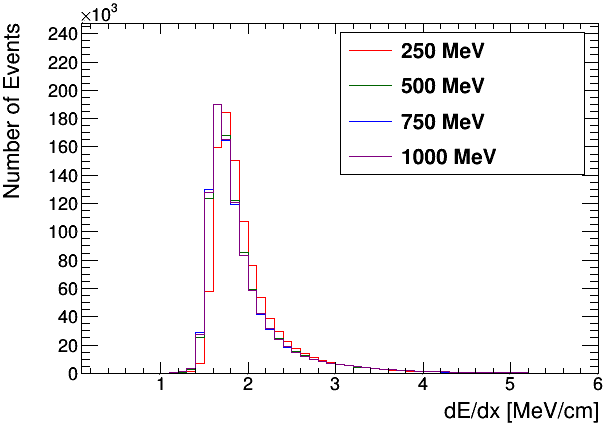
\includegraphics[height=65mm]{muons_per_mev_cm.png}
 \captionof{figure}{dE/dx of muons through single plastic bar assuming a density of plastic of 1\,g\,cm$^{-3}$. Mearuemnts for plastic are similar to carbon. For carbon $\sim$ 2\,MeV\,cm$^{-1}$ is expected for dE/dx {\cite{pdg_passage}. Mean dE/dx for 250\,MeV, 500\,MeV, 750\,MeV, 1000\,MeV are respectively 1.9907 $\pm$  0.0005\,MeV\,cm$^{-1}$, 1.9387 $\pm$  0.0005\,MeV\,cm$^{-1}$, 1.9374 $\pm$  0.0005 MeV\,cm$^{-1}$, 1.9407 $\pm$  0.0005 MeV\,cm$^{-1}$.\\}}
 \label{mev_per_cm_muons}
\end{Figure}

Positrons and muons were priority as positrons are produced during inverse-beta decay (equation \ref{inverse_beta_decay}) and muons (as previously mentioned) are a large background component. When simulating cosmic muons close to 20\,MeV the general trend of more energy being deposited at lower energies stops as shown in figure \ref{muon_0_250}. The cosmic muons no longer acted as MIPs, and were hard scattering off of the TiO$_2$ coating. An investigation into other particles was briefly conducted to determine the effects of this scattering, protons and pions were also simulated to determine this scattering at varying masses. The full list of particles and their anti-particles was therefore: e$^-$,e$^+$, $\pi ^+$, $\pi ^-$, $p$,  $\overline{p}$, $\mu $, $\overline{\mu}$.
\\

\begin{Figure}
 \centering
 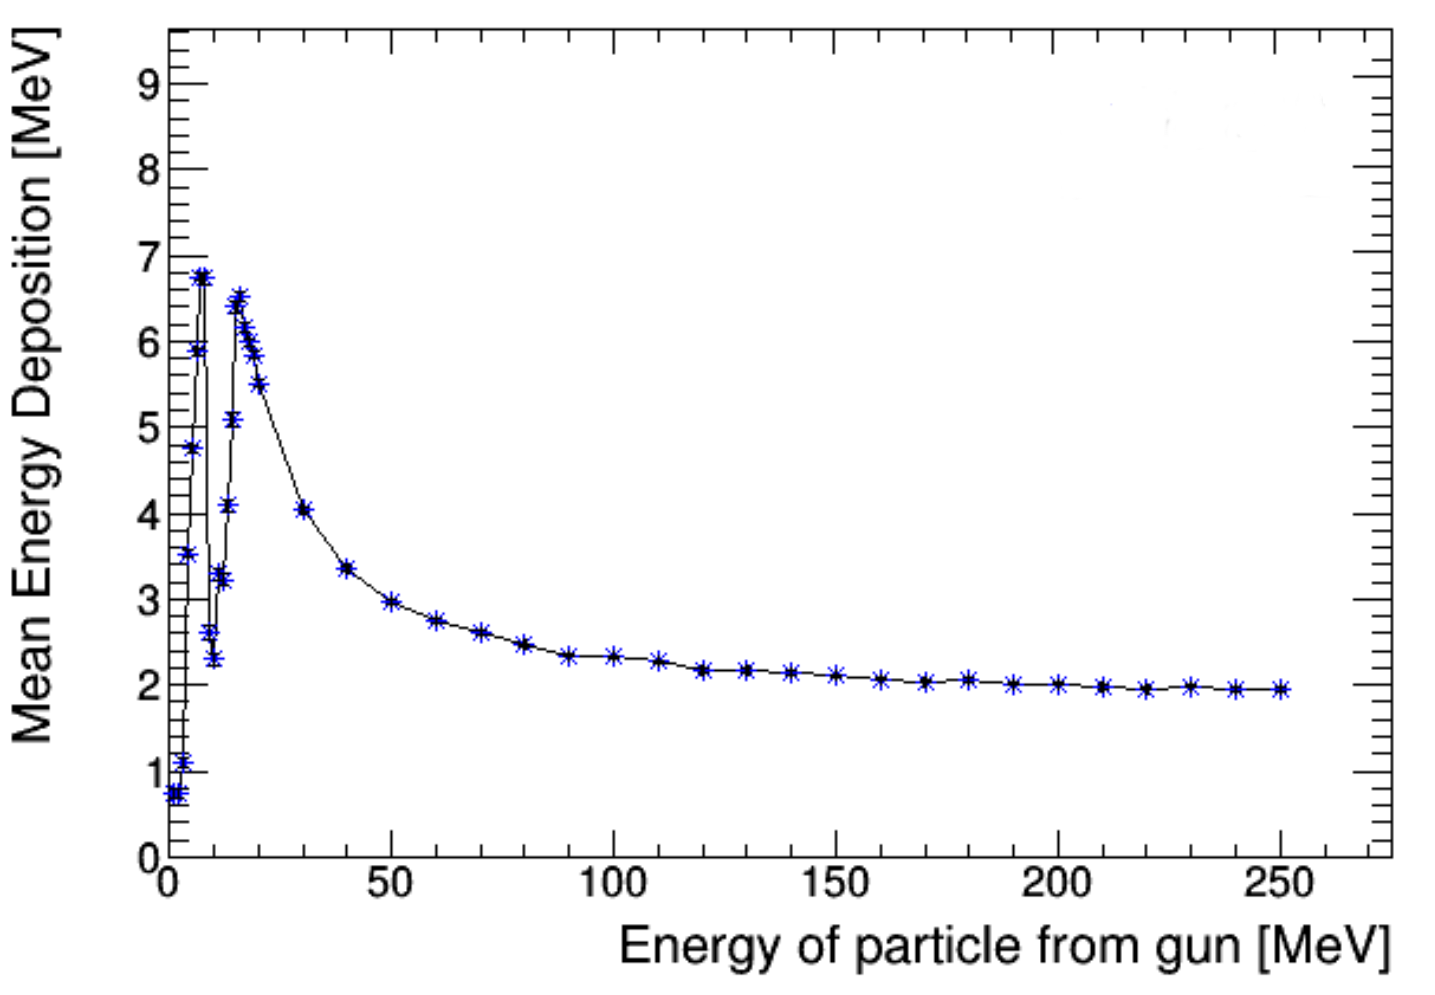
\includegraphics[height=65mm]{Muon_TiO2_med_eng.png}
 \captionof{figure}{Muon mean energy deposition in active component of the single bar, the sharp decrease in the energy deposited and varying deposition below 20\,MeV was due to the TiO$_2$ coating absorbing muons at lower energies.\\} 
 \label{muon_0_250}
\end{Figure}

%May want to mention muon stopping in bars and how important that was. Also make it clear that we have changed to dE/dx

By varying the percentage of TiO$_2$ in the 0.025\,mm coating that surrounds every bar it was possible to observe the effect of the scattering on simulated particles. In figure \ref{muon_tio2_per} a sharp increase in dE/dx happens at higher energies for higher percentages of TiO$_2$, a denser coating removes more energy, as expected. The effect on positrons is minimal until $<$ 2\,MeV as seen in figure \ref{pos_tio2_per}, this is due to their low rest mass. Occasionally they will interact directly with the nucleus, this significant variation causes the larger errors seen in figure \ref{pos_tio2_per} at certain points, for example at 40\,\% TiO$_2$ 12\,MeV. Protons can be produced in the VIDARR detector from fast neutrons, a potential source of noise from reactors, figure \ref{proton_tio2_per} shows proton dE/dx varying with TiO$_2$ percentage. Figure \ref{proton_tio2_per} shows how significant the effect of rest mass on the coating is, the protons show a much clearer loss of energy than muons or positrons and scales with TiO$_2$ percentage.


\begin{figure}[H]
\centering
\begin{subfigure}{.5\textwidth}
  \centering
  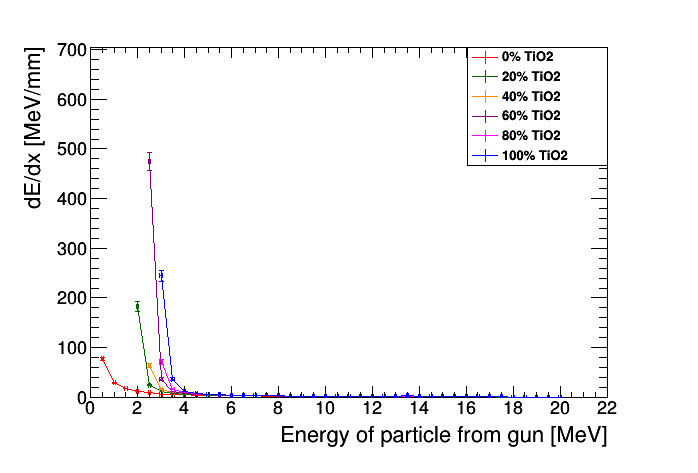
\includegraphics[width=\linewidth]{muon_TiO2__.png}
  \captionsetup{width=.9\linewidth}
  \caption{Muons with varying TiO$_2$ percentage in coating.}
  \label{muon_tio2_per}
\end{subfigure}%
\begin{subfigure}{.5\textwidth}
  \centering
  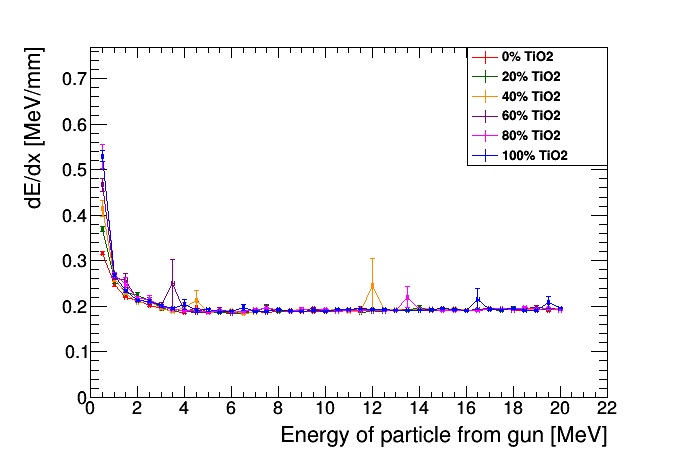
\includegraphics[width=\linewidth]{positron_TiO2__.png}
  \captionsetup{width=.9\linewidth}
  \caption{positrons with varying TiO$_2$ percentage in coating.}
  \label{pos_tio2_per}
\end{subfigure}
\caption{Positrons and muons with varying TiO$_2$ percentage in coating. TiO$_2$ coating ranging from 0\,\%-100\,\% with 20\,\% intervals. The effect on the muons is only observable below 4\,MeV whilst positrons are uneffected by the TiO$_2$}
\label{muon_pos_tio2_per}
\end{figure}

\begin{Figure}
 \centering
 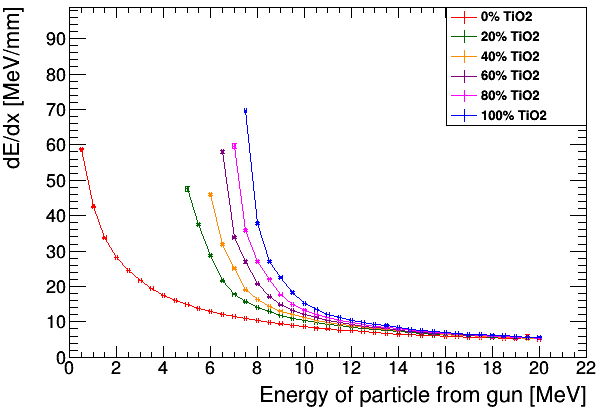
\includegraphics[height=71mm]{proton_TiO2__.png}
 \captionof{figure}{Protons with varying TiO$_2$ percentage in coating. TiO$_2$ coating ranging from 0\,\%-100\,\% with 20\,\% intervals. Protons are highly effected by the TiO$_2$.\\} %~can be used as a kind of place holder in latex
 \label{proton_tio2_per}
\end{Figure}

Muons are a potential calibration source, they are a constant source of events that do not require a reactor to be detected. Understanding their stopping behaviour and energy deposition in the detector and how much of an effect the coating will have on them with additional rest mass effects also being accounted for allows for increased understanding of their behaviour in our detector, making muons more useful for calibration. The effect on positrons is very small but will be noticeable at lower energies and the effect of the coating on protons is significant, and will help constrain them to s single bar. The errors for figures \ref{muon_0_250}, \ref{muon_pos_tio2_per}, \ref{proton_tio2_per} were standard error on the mean, each point on those figures represents the mean of 1000 points.

\subsection{Full Detector Model}
The full detector model is a representation of the detectors physical quantities, the materials and dimensions of the VIDARR detector. The full optical model of the detector is ignored in this type of simulation, this is to understand the deposition inside the detector and to improve the speed of the simulation. Optical properties are simulation intensive, as at every step the simulation must determine whether photons are produced and how they interact at every step in the detector or bar. Instead, the bar will be characterised by one of the other collaborators on VIDARR (George Holt) and then the photon response in the simulation of the single bar will be mapped on the full detector simulation using a photon function. This should give an accuracy comparable to full Monte Carlo simulation with significantly lower simulation time.
\\\\The full detector model, simulates the inverse $\beta$ decay caused by an $\overline{\nu_{e}}$ by simulating a prompt positron that occurs randomly inside the detector. The neutron is simulated by firing at the same time and position as positron but takes $\sim$ 10 $\mu$s to be thermalised and captured by the Gd, this is an accurate facsimile of how an $\overline{\nu_{e}}$ would behave inside our detector. The cross-section of an $\overline{\nu_{e}}$ is O $\sim$ 10$^{-42}$ cm$^2$ \cite{vogel_beacom_nu_cross} so not directly simulating it is necessary in these simulations, as Geant 4 is not well suited to small cross section interactions.
\\\\ The full simulation of the 2660 channels can be seen in figure \ref{2730_chan_det}. The simulation differentiates between neutrons and positrons by recording their particle data group particle id (PdgId) \cite{pdg_paper}, at present the electronics of the detector are not simulated, but their effect is expected to be minimal. The simulation can already begin to flag some events as ``ambiguous" when the neutron and the positron are detected within the same bar within 10 $\mu$s of each other.\\\\
\begin{Figure}
 \centering
 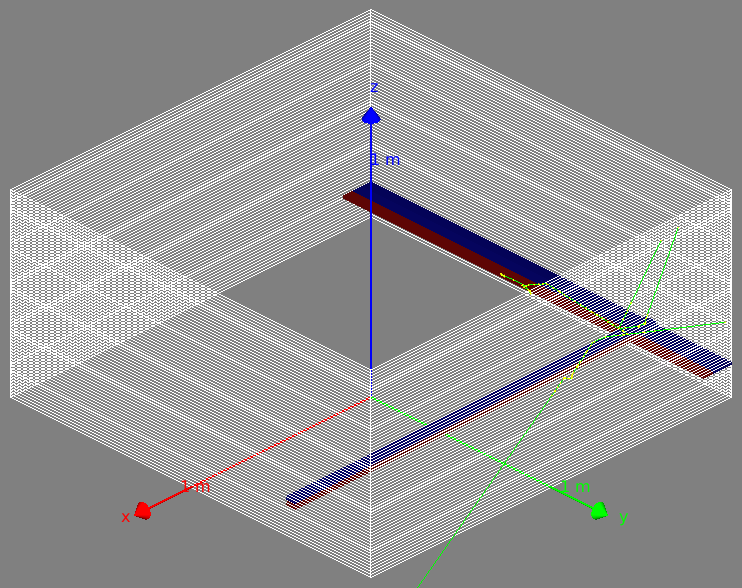
\includegraphics[height=71mm]{full_detector_2730_channels.png}
 \captionof{figure}{An inverse beta decay in the simulated 2660 channelled detector. Blue represents neutron hits and red represents positron hits, the path of the particle tracks are shown in green.\\} %~can be used as a kind of place holder in latex
 \label{2730_chan_det}
\end{Figure}


\section{Modelled efficiency}
Efficiency can be split up into multiple components, detection and reconstruction efficiency. The detector will use positrons to determine the position of the $\overline{\nu_{e}}$ as it only hits $\sim$ 2 adjacent bars. The efficiency for the $e^+$s is expected to be very close to 100\,\% as its highly probable they will annihilate within the detector, and do not travel far. Even when $e^+$s leave the detector as they are charged particles it is highly likely they will deposit some of their energy in the detector and will still be seen. However it is the neutrons that the detector will trigger on. It will detect the Gd $\gamma$ cascade and then look backwards in a buffer to find the $e^+$ and determine weather a $\overline{\nu_e}$ event occurred. The trigger will activate on the number of bars hit and the reconstructed energies from two different thresholds (0.1\,MeV and 0.75\,MeV). However the energy must be smeared using a statistical model, in order to recreate a more accurate cut. As these trigger cuts are the only cuts on the neutrons their efficiency is currently the efficiency of the neutrons in the detector.

\subsection{Statistics and Errors}
The uncertainties on the simulated data are dominated by counting (Poisson) statistics, the error for a Poisson distribution is the~ $\sqrt[]{N}$, where $N$ is the number of events. In simulated data, providing that the statistics are high ($\sim 10^6$ and above) these errors as a fraction of the total simulated events become insignificant. For example, and $10^6$ will have an error of 1000 (0.1\,\% error) which was deemed sufficient for the full detector simulation. The statistical uncertainties on the simulated data are not representative of the systematic error on the simulation, which is why they have not been included in any of the plots.\\

The other errors that are derived from the Poisson statistics, such as the standard error on the mean ($\sigma/\sqrt[]{N}$) are equally small, as in figure {\ref{Recon_gen_ele_pos}} where the mentioned errors are O $\sim 10^{-3}\,\% - 10^{-4}\,\%$). Efficiency errors are also insignificant as they come from the equation $\Delta z = 100 \times z \sqrt[]{(\Delta x / x)^2 + (\Delta y / y)^2}$ where $\Delta x$ and $\Delta y$ are $\sqrt[]{N}$ and x and y are N in figure {\ref{2000_3000_p_secs}} this results in errors of $10^{-3}$\,\%, too small to be seen in the figure.\\

More accurate errors could be determined through comparisons of measured data, for example an upper and lower bound on the simulated values could be quantified using the errors of the photon electron conversion (25.3\,\pm\,0.1) in future. Once a more in-depth comparison with measured data has been done the errors on the simulation can be accurately determined, instead of using systematic errors that give a higher accuracy than is realistic. 

\subsection{Positron efficiency}
Positrons are antimatter, their annihilation with electrons means that they are unlikely to penetrate very far outside of the detector geometry, providing their energies are $<$ 10\,MeV, only those at the very edge can escape the detector. So the detection efficiency is very high for positrons as most of them will annihilate inside the detector, their penetrating distance is $\sim$ 2cm. For 2660 bars the detection efficiency of the deposited/truth is $\sim$ 99\,\%, this means that very few $e^+$ are physically escaping the detector, as expected. 
\\\\ The results for the 2660 channels $e^+$ truth, deposited, escaped and reconstructed can be seen in figure \ref{e+_3000_effs_thresh_0.1}, the large peak at $\sim$ 0.336 MeV is the Compton edge for the annihilation $\gamma$s of the positrons. Two million 511 keV $\gamma$ rays are produced in the detector in figure \ref{e+_3000_effs_thresh_0.1} as we simulate 1 million positrons, however, most $\gamma$ rays also interact at the same time as the positrons in the bars, so their energy is often added to the positron's energy as well. The peak at $\sim$ 0.336MeV has more events than any of the other bins, however, this only represents $\sim$ 0.65\% of the $\gamma$ rays that are fired into the detector. The others deposit their energy into other non-active components of the simulated detector or at the same time as the positrons deposit their energy into the active scintillating bars of the simulated detector.

\begin{Figure}
 \centering
 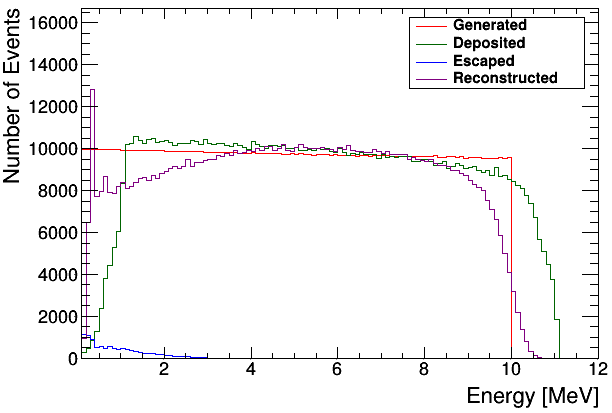
\includegraphics[height=71mm]{truth_inside_outside_and_seen_e+_thresh0_1.png}
 \captionof{figure}{Histogram of positron energies in simulated upgraded detector (2660 bars, 0.1\,MeV Threshold), bins of 0.1\,MeV, $10^6$ events.\\} %~can be used as a kind of place holder in latex
 \label{e+_3000_effs_thresh_0.1}
\end{Figure}

If we increase the precision of figure \ref{e+_3000_effs_thresh_0.1} from 0.1\,MeV bins to 0.01\,MeV bins and focus on the reconstructed signal it's possible to show the peak shape in finer detail. This finer binning is illustrated in figure \ref{Compton_edge_cuts_and_no_cuts} showing the positron energies between 0\,MeV-1\,MeV with and without cuts, it is mostly the adjacency cut that determines the proximity of the events that has such a significant impact on the peak in figure \ref{Compton_edge_cuts_and_no_cuts}. This is because the Compton electrons (and their corresponding $\gamma$s) produced from positron events are more effectively removed by an adjacency cut (where two or more hit bars must be next to each other in $x$, $y$ or $z$ plane). As the positrons annihilate closer to the edge of the bar than the centre $\gamma$s from annihilation are more likely to hit an adjacent bar so the 511\,keV are successfully seen in figure \ref{Compton_edge_cuts_and_no_cuts} at 0.336\,MeV.

\begin{Figure}
 \centering
 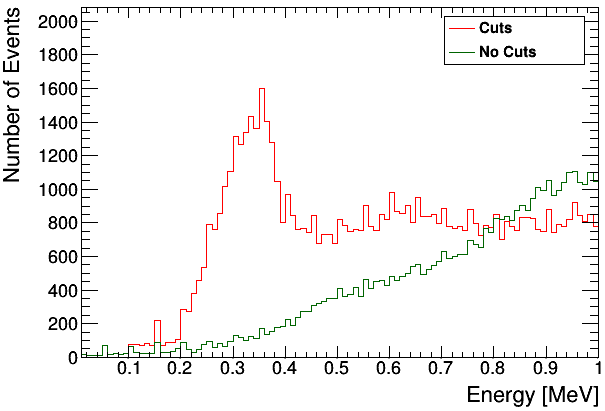
\includegraphics[height=71mm]{compton_edge_no_and_checks.png}
 \captionof{figure}{Histogram of reconstructed positron energies in simulated upgraded detector from 0-1 MeV with bins of 0.01MeV (ten times finer binning than figure \ref{e+_3000_effs_thresh_0.1}).\\} %~can be used as a kind of place holder in latex
 \label{Compton_edge_cuts_and_no_cuts}
\end{Figure}

The bars and scintillating fibres in the upgraded detector remain the same from the original, the electronics are not simulated at this time (except the threshold of 100 keV). Both the upgraded and original detector simulation used $10^6$ to minimise statistical uncertainties. Apart from the number of layers increasing from 49 to 70 between the simulations the threshold which in figure \ref{e+_3000_effs_thresh_0.1} had been 0.1 MeV was 0.5 MeV for the original detector simulation seen in figure \ref{e+_2000_effs_thresh_0.5}. The higher threshold on the original simulated detector prevents any potential Compton edge effect from being seen which is why it is not visible in figure \ref{e+_2000_effs_thresh_0.5}.     

\begin{Figure}
 \centering
 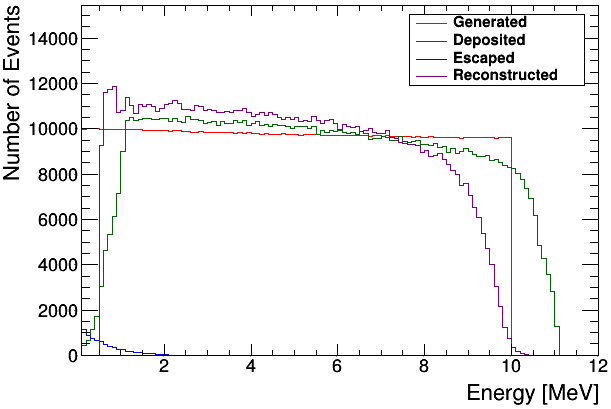
\includegraphics[height=71mm]{inverseBRun2000_data_storage_thresh0_5.png}
 \captionof{figure}{Histogram of reconstructed positron energies in simulated original detector (1862 bars, 0.5\,MeV Threshold), bins of 0.1MeV, $10^6$ events.\\} %~can be used as a kind of place holder in latex
 \label{e+_2000_effs_thresh_0.5}
\end{Figure}

Figures \ref{e+_3000_effs_thresh_0.1} and \ref{e+_2000_effs_thresh_0.5} are oversimplified, energies from positrons will be deposited in the detector with the energies shown. But the simulation includes all signals from the positron including the annihilation gamma rays, this means that the signals have a component of their energy associated with the 511\,keV $\gamma$ peak. In reality, it will be quite difficult to distinguish the low energy $\gamma$ rays from the background noise and smearing of the detector. The simulation represents an idealised version of the reconstruction energy, there is no smearing or noise, the reconstruction code will add together all events that are adjacent to the main event. But it is unclear if that is a feasible cut for the real life detector. The spectrum that the 2 $\times 10^6$  positrons produce in our detector is shown in figure \ref{gamma_spectra}. There is a clear peak in the gamma spectra at $\sim$ 0.336\,MeV which is where we would expect a Compton peak to occur for 511\,keV gamma rays. 
%might need to go into more theory here, I've got to explain why we see the 3.36mev peak in the plastic, maybe even a bit before here... 


\begin{Figure}
 \centering
 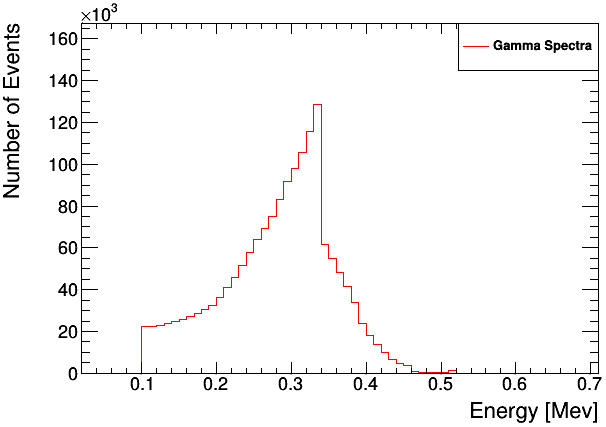
\includegraphics[height=71mm]{511centre_run_data_storage_root.png}
 \captionof{figure}{Reconstructed energy in the detector for the 511\,keV $\gamma$s that occur when $e^+$s annihilate.\\} %~can be used as a kind of place holder in latex
 \label{gamma_spectra}
\end{Figure}

Until noise is simulated it is difficult to discern if the secondaries can be distinguished from the background noise. At present the simulation does not include noise for $e^+$s, as the upgraded detector has not yet been constructed so no measurement can be taken. The simulation's priority is to determine the physical factors affecting the efficiency of the detector and comparison of those physical factors between the original 1862 barred detector and the upgraded 2660 barred detector. The hit efficiencies of positrons across the energy range expected for $e^+$ (1\,MeV - 10\,MeV) can be seen in figures \ref{2000_p_sec} and \ref{3000_p_sec}.

\begin{figure}[H]
\centering
\begin{subfigure}{.5\textwidth}
  \centering
  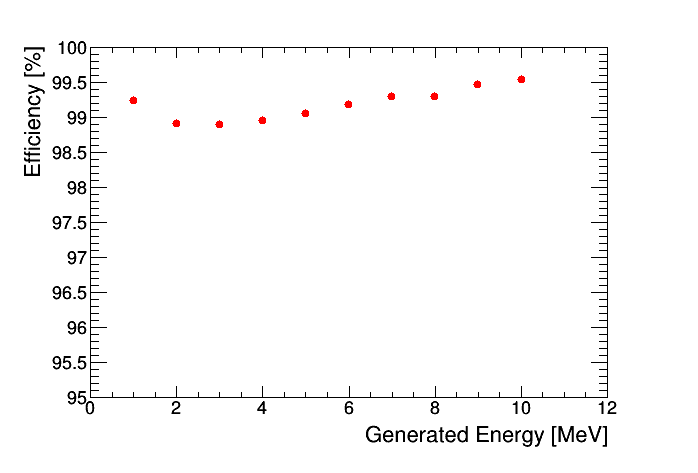
\includegraphics[width=\linewidth]{2000_1-10MeV_sec_p_spread_run.png}
  \captionsetup{width=.9\linewidth}
  \caption{Positrons hit efficiencies in the 1862 barred detector $\sim$ 99\,\% of positrons are detected.}
  \label{2000_p_sec}
\end{subfigure}%
\begin{subfigure}{.5\textwidth}
  \centering
  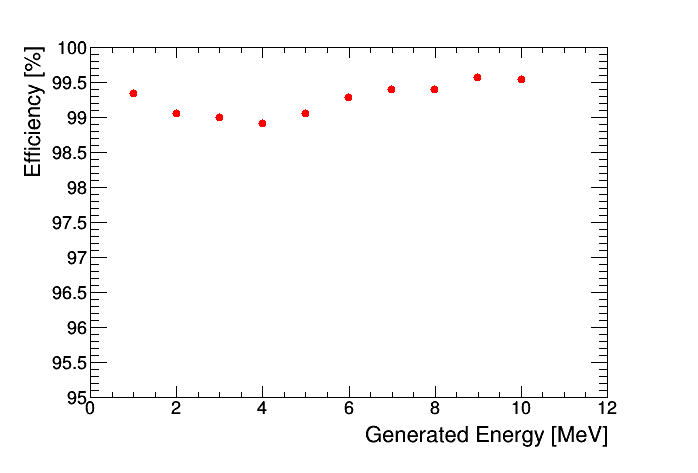
\includegraphics[width=\linewidth]{3000_1-10MeV_sec_p_spread_run.png}
  \captionsetup{width=.9\linewidth}
  \caption{Positrons hit efficiencies in the 2660 barred detector $\sim$ 99\,\% of positrons are detected.}
  \label{3000_p_sec}
\end{subfigure}
\caption{Positron hit efficiencies for the original 1862 barred detector and the upgraded 2660 barred detector both have $\sim$ 99\,\% efficiencies are similar in both errors are too small to be shown Generated energy O $\sim$ $10^{-8}$ efficiency error O $\sim$ $10^{-3}$.}
\label{2000_3000_p_secs}
\end{figure}

Figures \ref{2000_p_sec} and \ref{3000_p_sec} show that there is no significant difference between the detection efficiency between the original 1862 barred detector and the upgraded 2660 barred detector. This is due to the small interaction length of the positrons ($\sim$ 2\,cm) inside the detector. Only those positrons produced $\lesssim$ 2\,cm can escape the detector, but even these will still deposit some energy and will still be seen by the detector resulting in an overall e$^+$ positron efficiency of $\sim$ 99\%. 

\subsection{Reconstructed Energy Response for Simulated $e^-$ and $e^+$}
By generating positrons and electrons with specific energies from 1-10\,MeV with 1\,MeV Intervals, as was done in figures \ref{2000_p_sec} and \ref{3000_p_sec}, we can then then take the mean reconstructed energy (E$_\textrm{{reco}}$) and compare it to the generated energy (E$_\textrm{{gen}}$). The energy response of the detector is mostly linear as can be seen in figure \ref{Recon_gen_ele_pos}, a small fraction of the energy is lost in the detector, most of it is successfully reconstructed. In figure \ref{Recon_gen_ele_pos} the electrons are a more accurate representation of the detector's energy response as they do not produce annihilation $\gamma$-rays in the detector, so the energy loss is most clearly seen with them. At low E$_\textrm{{gen}}$ $e^+$ E$_\textrm{{gen}}$ $<$ $e^+$ E$_\textrm{{reco}}$ due to the extra 511\,keV energy produced by the $e^+$ annihilation in the detector. As E$_\textrm{{gen}}$ increases the number bars hit increases, more energy as a percentage is deposited into the gadolinium sheets and TiO$_2$ of the VIDARR detector resulting in higher E$_\textrm{{reco}}$ loss at higher E$_\textrm{{gen}}$ for both $e^+$s and $e^-$s.  

\begin{Figure}
 \centering
 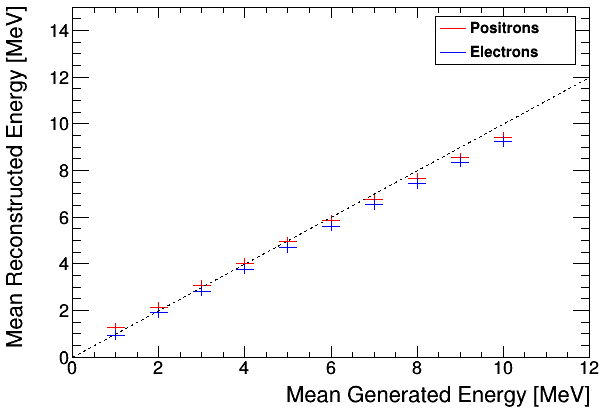
\includegraphics[height=71mm]{Recon_vs_gen_e-_e+.png}
 \captionof{figure}{Energy response of the simulated detector for both electrons and positrons in the full detector in comparison to E$_\textrm{{reco}}$ = E$_\textrm{{gen}}$. The positron's annihilation $\gamma$s causes E$_\textrm{{reco}}$ $>$ E$_\textrm{{reco}}$ at low generated energies. Reconstructed error O $\sim$ $10^{-3}$\,MeV  and generated error O $\sim$ $10^{-8}$\,MeV, neither shown as they are both too small to be visible.}%~can be used as a kind of place holder in latex
 \label{Recon_gen_ele_pos}
\end{Figure} 

\subsection{Neutron Efficiency}
\subsubsection{Simulated Gadolinium Capture}
There are two models that are used for gadolinium capture in Geant 4 the first of these is a ``photon evaporation model", this model has a strong theoretical basis and produces energies that we can identify in gadolinium's spectra. The spectrum for this model can be seen in figure \ref{evap_gd}, whilst the individual $\gamma$ energies in this spectrum are consistent with Gd's prompt $\gamma$ spectra (prompt spectra can be seen in figure \ref{gd_prompt_gs}) the summed $\gamma$s do not match the prompt $\gamma$ spectra a comparison of which can be seen in figure \ref{comparison_gd_gammas}. 

\begin{figure}[H]
\centering
\begin{subfigure}{.5\textwidth}
  \centering
  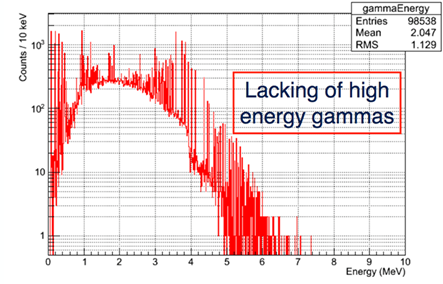
\includegraphics[width=\linewidth]{evaporation_gdmodel.png}
  \captionsetup{width=.9\linewidth}
  \caption{Individual $\gamma$ energies for the photon evaporation Gd model from \cite{Gd_models}.}
  \label{evap_gd}
\end{subfigure}%
\begin{subfigure}{.5\textwidth}
  \centering
  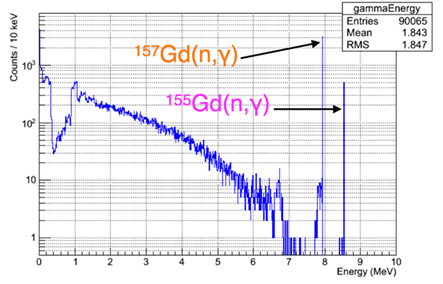
\includegraphics[width=\linewidth]{finalstate_gdmodel.png}
  \captionsetup{width=.9\linewidth}
  \caption{Individual $\gamma$ energies for the final state Gd model from \cite{Gd_models}.}
  \label{finalst_gd}
\end{subfigure}
\caption{Comparisons of the gadolinium models used in Geant4, \ref{evap_gd} shows evaporation model, \ref{finalst_gd} shows final state model, from \cite{Gd_models}.}
\label{evap_fnst_gd}
\end{figure}

\begin{Figure}
 \centering
 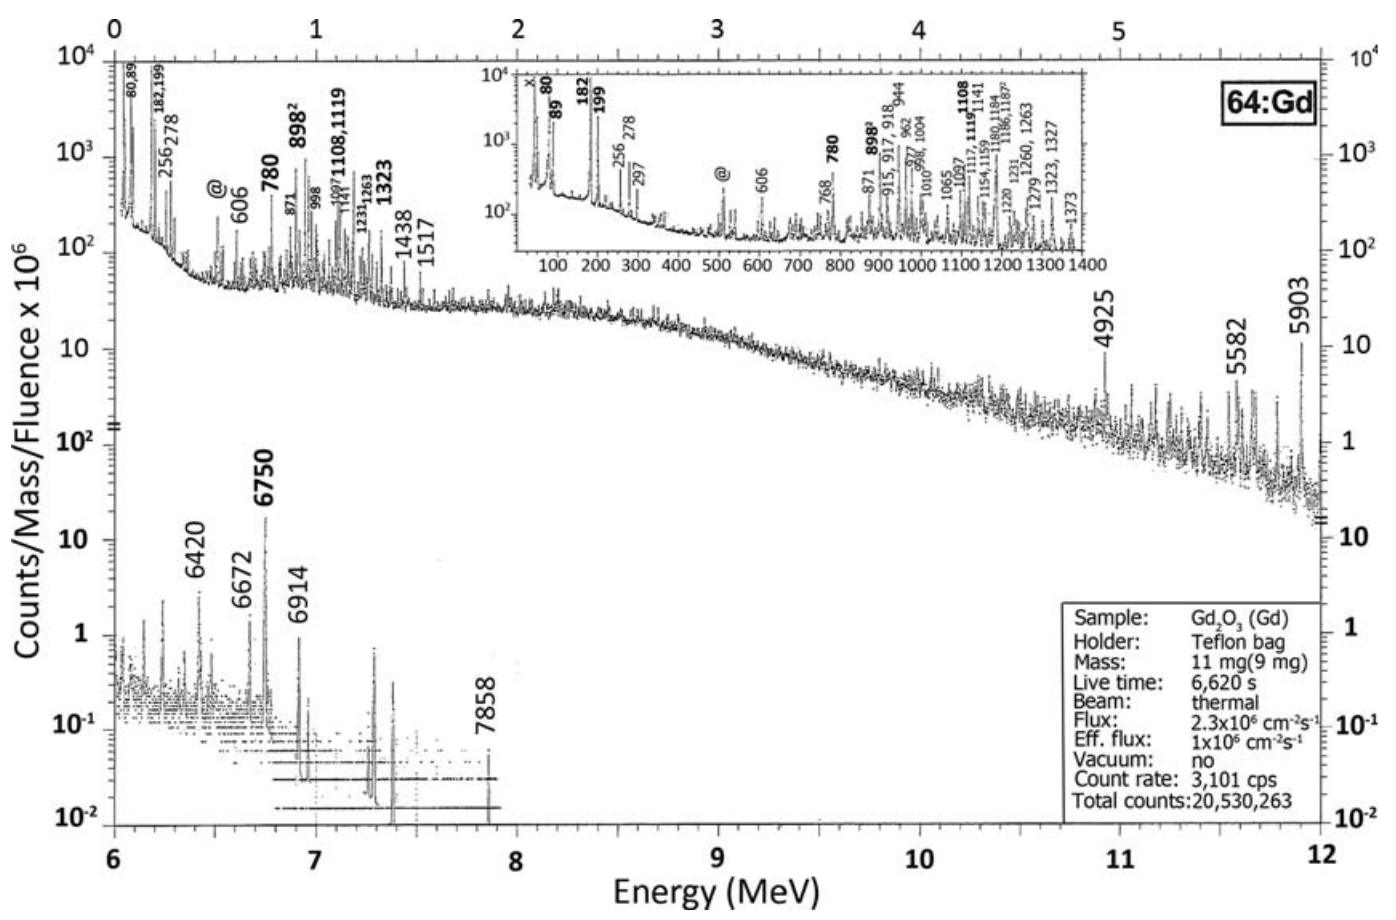
\includegraphics[height=71mm]{gd_prompt.png}
 \captionof{figure}{The measured neutron-induced $\gamma$ rays from natural Gd from \cite{prompt_gd_gamma_paper} it is this spectra that is then compared with figures \ref{evap_gd} and \ref{finalst_gd} in figure \ref{comparison_gd_gammas}. \\} %~can be used as a kind of place holder in latex
 \label{gd_prompt_gs}
\end{Figure} 

\begin{Figure}
 \centering
 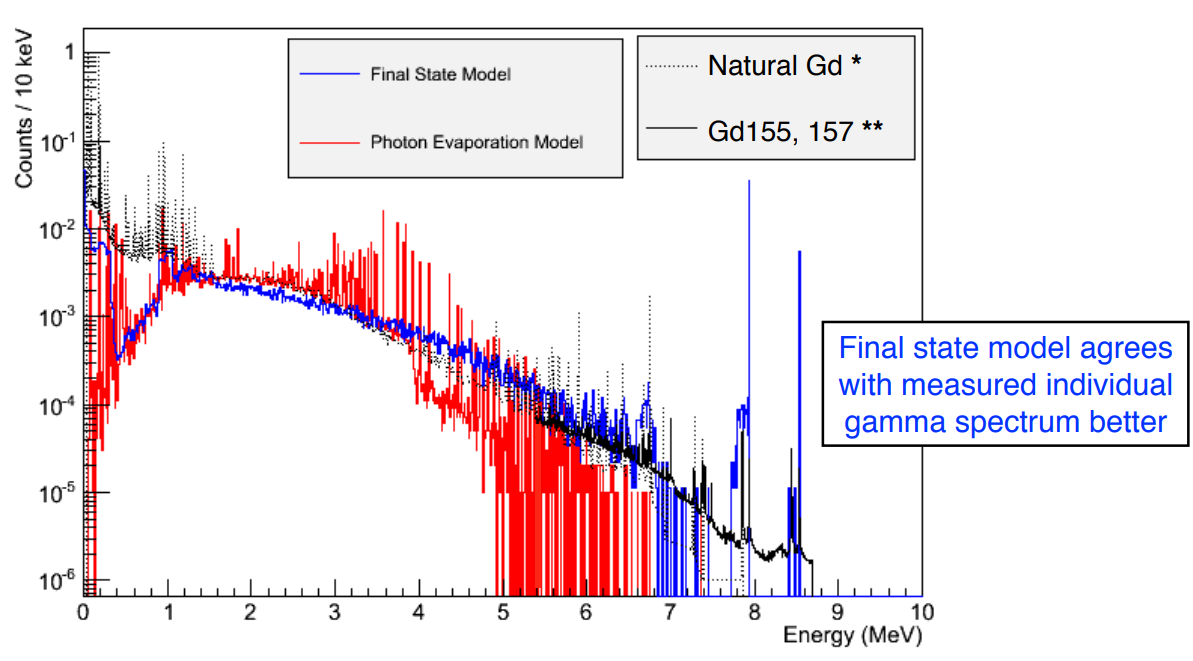
\includegraphics[height=71mm]{comparison_of_gd_gammas.png}
 \captionof{figure}{Comparison of Gd $\gamma$ spectra with photon evaporation in red, final state in blue and the measured spectra in black, the black is most similar to the final state, from \cite{Gd_models}. \\} %~can be used as a kind of place holder in latex
 \label{comparison_gd_gammas}
\end{Figure} 

The alternative model is the ``final-state'' model, in Geant4 this can mean multiple implementations: ``Three classes of models are distinguished for modelling final states. There are models that are largely based on evaluated or measured data, models that are predominantly based on parameterisations and extrapolation of experimental data under some theoretical assumptions, and models that are predominantly based on theory'' \cite{geant4_ref}. The final-state model is therefore the model that matches the final state of the data, however this requires the creation of $\gamma$s that are potentially un-physical. In figure \ref{finalst_gd} we see the creation $\gamma$s at $\sim$ 8\,MeV for $^{157}$Gd and $\sim$ 8.5\,MeV for $^{155}$Gd, at present there is no physical evidence for these $\gamma$s to be directly produced from Gd. It is possible that such high energy $\gamma$s do exist but their high energy would make them difficult to confirm via current detection methods, the final state method also breaks the conservation of energy. However as figure \ref{comparison_gd_gammas} shows the measured spectra is more closely followed by final state than by photon evaporation.


\subsubsection{Photon Equivalent Units}
The VIDARR detector does not measure energy directly, the scintillating plastic and WLS fibres outputs photons that are detected by MPPCs. The reconstruction of the signal from the simulation emulates this by using a photon equivalent (PEq) conversion. This is to determine the resolution of the results, the detector measures photons in integers, the number of photons per MeV was 25.3\,\pm\,0.1 and was determined by measurements done by George Holt who also works on the VIDARR collaboration. Invert 25 \pm 0.1 and this gives 0.04 \pm 0.002\,MeV per photon, every simulated data point must be converted to photons giving a binning of 0.04\,MeV binning, this binning or resolution is the PEq for the VIDARR detector. %I feel like I should be saying more here, but I really have no idea what else to add...

\subsubsection{Statistical Model}
The simulation must also represent the counting statistics of the MPPCs for different energies. The physical effect of the MPPC counting photons can be represented as counting statistics for a small probability of success. These counting statistics are represented Poisson distribution shown in equation \ref{possion_equation} when we have a small constant probability of success. For this distribution $pn = \overline{x}$ where $\overline{x}$ is the expectation value, substituting this into equation \ref{possion_equation} we get equation \ref{possion_equation_expct}. The evaluation of the variance in equation \ref{possion_var} means that the standard deviation is $\sigma=\sqrt[]{\overline{x}}$ \cite{rad_det_and_meas}.

\begin{equation}
P(x) = \frac{(pn)^x e^{-pn}}{x!}  
\label{possion_equation}
\end{equation}

\begin{equation}
P(x) = \frac{(\overline{x})^x e^{-\overline{x}}}{x!}  
\label{possion_equation_expct}
\end{equation}

\begin{equation}
\sigma ^2 \equiv \sum_{x=0}^{n} (x-\overline{x})^2 P(x) = pn = \overline{x} 
\label{possion_var}
\end{equation}

The equation for a Gaussian distribution is shown in equation \ref{guassian_expect}, the standard deviation for both of the distributions is $\sigma=\sqrt[]{\overline{x}}$. When the statistics of the Poisson distribution are high enough then it can be approximated to a Gaussian distribution. Due to the $x!$ in equations \ref{possion_equation} and \ref{possion_equation_expct} this approximation is useful as it decreases computational intensity. The tolerance for this was set to 99.9\,\% of the event in the Poisson distribution being above 2 events or more, this occurs at a mean of 10 photons. After a mean of 10 photons the Gaussian distribution is used instead. The distribution of the smearing for 10 photons can be seen in figure \ref{10phot_pois_gaus}, a slight skew in the Poisson is visible but the distributions approximate. 2 photons is the limit the detector will trigger on. 
\begin{equation}
P(x) = \frac{1}{\sigma \sqrt[]{2 \pi}} \exp \left(-\frac{1}{2}\left(\frac{x-\overline{x}}{\sigma}\right)^{2}\right)
\label{guassian_expect}
\end{equation}

\begin{Figure}
 \centering
 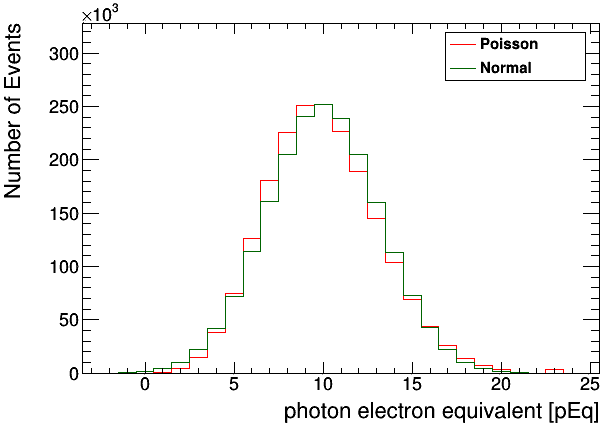
\includegraphics[height=71mm]{10phot.png}
 \captionof{figure}{The statistical (counting) function at 10 photons, 99.9\,\% of the simulated data in Poisson distribution has 2 or more photons ($\geq$ 0.08\,MeV).} %~can be used as a kind of place holder in latex
 \label{10phot_pois_gaus}
\end{Figure}


\subsubsection{Containment of Gd $\gamma$ Cascade}
The neutrons do not release any ionising radiation as they are neutral particles. The kinetic energy expected from inverse beta decay neutrons is thermal (0.025\,eV -- 0.075\,eV). The detector will only detect neutrons if they are captured by the Gd, or if their energies are high enough to start showering. Therefore direct energy measurements anologus to positron and muon efficiency measurements are not applicable as the energy of the neutrons is not directly measured. Instead the $\gamma$ cascade from the Gd is measured. The percentage of escaping neutrons in the detector gives $\sim$ 2\,\% for 1832 bars and $\sim$ 1.7\,\% for 2660 bars. If we plot the energy of the reconstructed $\gamma$ cascade for both the 1862 bars detector and the 2660 bars detector with no smearing figures \ref{sub_2000_gd_h} and \ref{sub_3000_gd_h} are produced. Applying the smearing due to the quantised MPPC response results in figures \ref{sub_2000_gd_h_peq}, \ref{sub_3000_gd_h_peq} are produced. 

\begin{figure}[H]
\centering
\begin{subfigure}{.5\textwidth}
  \centering
  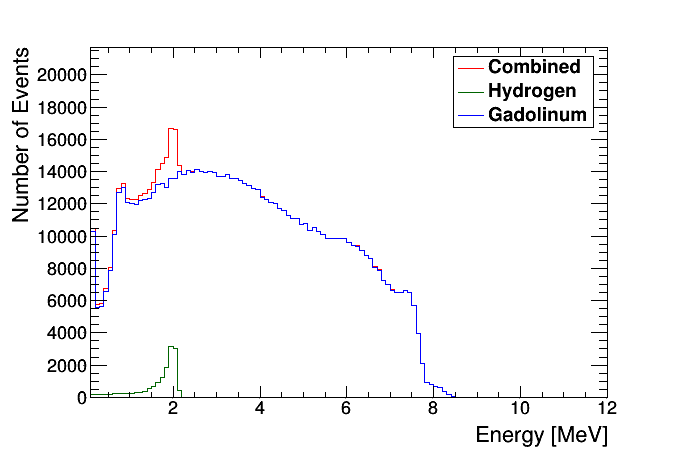
\includegraphics[width=\linewidth]{neutron_2000_bars_Gd_H.png}
  \captionsetup{width=.9\linewidth}
  \caption{Reconstructed energies of $\gamma$s produced from H and the Gd cascade produced by neutrons in the 1862 bars detector.}
  \label{sub_2000_gd_h}
\end{subfigure}%
\begin{subfigure}{.5\textwidth}
  \centering
  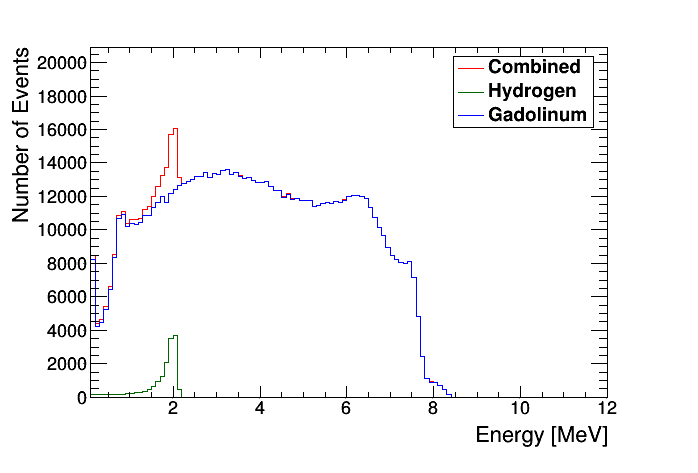
\includegraphics[width=\linewidth]{neutron_3000_bars_Gd_H.png}
  \captionsetup{width=.9\linewidth}
  \caption{Reconstructed energies of $\gamma$s produced from H and the Gd cascade produced by neutrons in the 2660 bars detector.}
  \label{sub_3000_gd_h}
\end{subfigure}
\caption{Gadolinium and Hydrogen reconstructed energies for 1862 and 2660 bars after absorbing neutrons (no smearing).}
\label{3000_2000_gd_h}
\end{figure}

The efficiencies between figures \ref{sub_2000_gd_h_peq} and \ref{sub_3000_gd_h_peq} are very similar, $\sim$ 86\,\% for 1862 bars and $\sim$ 88\,\% for 2660 bars. But when looking at figures \ref{sub_2000_gd_h} and \ref{sub_3000_gd_h} and figures \ref{sub_2000_gd_h_peq} and \ref{sub_3000_gd_h_peq} above 6\,MeV (150\,pEq) the spectra appear to have more than a 2\,\% improvement when comparing 1862 to 2660 bars. This is due to the improvement in containment seen in figure \ref{containment_comparison}. The containment is defined as the percentage of $\frac{E_\gamma reco}{E_\gamma gen}$. In figure \ref{containment_comparison} the average containment was $\sim$ 48\,\% for 1862 bars and $\sim$ 53\,\% for 2660 bars, this is over twice the improvement seen in efficiency. But also the number of high quality events has improved significantly, in figure \ref{containment_comparison} between 70\,\% and 100\,\% we see peak containment at 85\,\% increase from $\sim$ 16000 in 1862 bars to $\sim$ 20000 in 2660 bars. This improvement in containment causes the significant improvement in the neutron spectrum between above 6\,MeV for figures \ref{sub_2000_gd_h} and \ref{sub_3000_gd_h} (150\,pEq for figures \ref{sub_2000_gd_h_peq} and \ref{sub_3000_gd_h_peq}). This also results in less noise at lower energies when upgrading to 2660 bars improving the potential for the hydrogen signal to be used as calibration. 

\begin{figure}[H]
\centering
\begin{subfigure}{.5\textwidth}
  \centering
  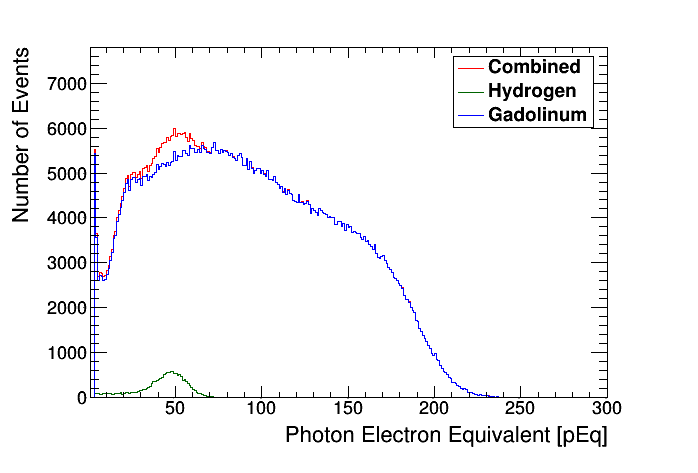
\includegraphics[width=\linewidth]{neutron_2000_bars_Gd_H_PEQ.png}
  \captionsetup{width=0.9\linewidth}
  \caption{Reconstructed energies of $\gamma$s produced from H and the Gd cascade produced by neutrons in the 1862 bars detector.}
  \label{sub_2000_gd_h_peq}
\end{subfigure}%
\begin{subfigure}{.5\textwidth}
  \centering
  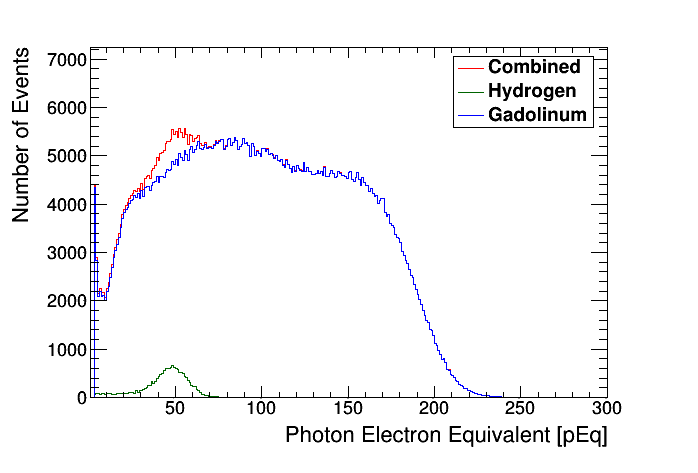
\includegraphics[width=\linewidth]{neutron_3000_bars_Gd_H_PEQ.png}
  \captionsetup{width=.9\linewidth}
  \caption{Reconstructed energies of $\gamma$s produced from H and the Gd cascade produced by neutrons in the 1862 bars detector.}
  \label{sub_3000_gd_h_peq}
\end{subfigure}
\caption{Gadolinum and Hydrogen reconstructed signals for 1862 and 2660 bars after absorbing neutrons (with smearing).}
\label{2000_3000_gd_h_peq}
\end{figure}

\begin{Figure}
 \centering
 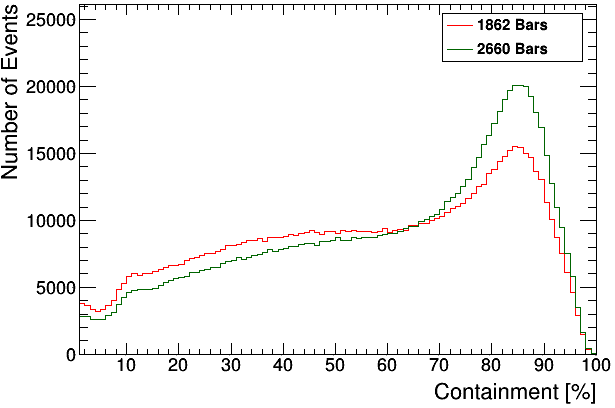
\includegraphics[height=71mm]{containment_Energy.png}
 \captionof{figure}{Quality of the containment of event energy in the 1862 bars detector and the 2660 bars detector where the containment is defined as the percentage of $\gamma$ cascade reconstructed energy compared to the $\gamma$ cascade generated energy.} %~can be used as a kind of place holder in latex
 \label{containment_comparison}
\end{Figure} 

\subsubsection{Threshold and Trigger for the upgraded VIDARR}\label{trigger_section_by_hand}
The upgraded VIDARR detector has the potential for two different triggers. A trigger is defined as a set of conditions that the electronics will notice if an event in the detector meets those conditions. A threshold is defined as the minimum energy that a hit inside a single bar must be greater than in order for the electronics to register a response. The conditions for the detector's trigger were set as two thresholds for individual bar hits by using this set up it may be possible to quickly discriminate between particle types. The neutron signature is what the electronics use to discern anti-neutrino events from the background, so the primary objective of the trigger is to separate the neutron events from all other events, to create a neutron trigger. Random background and noise has several sources, cosmic muons, Compton scattering via $e^-$s, and stray $\gamma$s. \\\\
Thresholds 0.1\,MeV and 0.75\,MeV were chosen as hits in a single bar are likely to differ between these two energies. The cuts for the threshold and trigger were determined by requiring a neutron acceptance of $\sim$ 70\,\% and that the neutrons and electrons would separate out, to maximise ``purity". The reconstructed energies from the two thresholds in figures \ref{2drecon_n_cut} and \ref{2drecon_e_cut} were clear 2d cuts as they varied significantly in both axes. However as figure \ref{thresholds_bars_hit} shows the numbers of bars hit varied significantly more in the 0.1\,MeV axis than in the 0.75\,MeV axis. So for the number of bars hit a 1d cut was deemed sufficient. The bar cut that met the previously mentioned criteria was 4 bars which figure \ref{4_bar_cut} shows. Theses cuts are ``either or'' which means that events in the detector must meet either one of the criteria in order to be recorded.%  The two thresholds tested were 0.10\,MeV and 0.75\,MeV the number of bars hit at the 0.75\,MeV for neutrons fell at a 63.6\,\% when over 2bars but the electron efficiency for the same cut was 60.8\,\%, the signals did not separate out.\\\\

\begin{Figure}
 \centering
 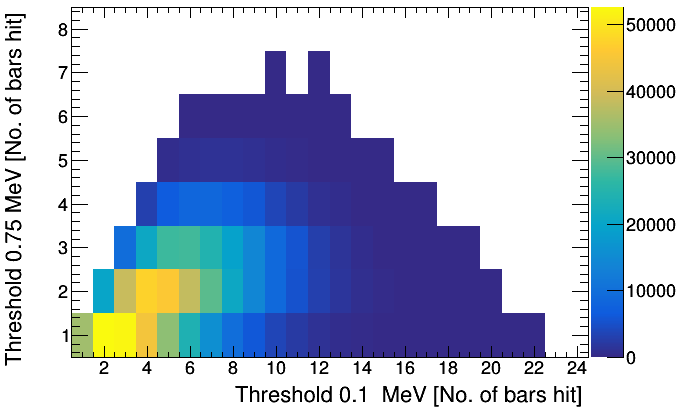
\includegraphics[height=71mm]{barsHitThr0_1_0_75.png}
 \captionof{figure}{Number of bars hit by neutrons for both thresholds in the 2660 barred detector the response varies significantly more in the Threshold 0.1\,MeV axis, suggesting that a 1D cut on the numbers of bars hit would be sufficient.\\} %~can be used as a kind of place holder in latex
 \label{thresholds_bars_hit}
\end{Figure} 

When applying a bar cut of $\geq$ 4 to the simulated neutron data at a threshold of 0.1\,MeV as seen in figure \ref{4bar_n_cut} the acceptance is 67.9\,\% and the same cut in figure \ref{4bar_e_cut} results in an $e^-$ acceptance of 16.2\,\%, which achieves a separation of the simulated data. Now we can introduce another cut, this time using the previously mentioned bar thresholds. The 2D rejection of the reconstructed $\gamma$ cascade energies took the form of a straight line with a gradient of 1 producing equation \ref{Recon_cut_eq}:
\begin{equation}
E_{\textrm{reco}}^{\textrm{0.75MeV}} \leq E_{\textrm{reco}}^{\textrm{0.1MeV}} - E_\textrm{intercept}
\label{Recon_cut_eq}
\end{equation}
All events that fulfil this condition are accepted leading to the line of rejection shown in figure \ref{thr_thr_cut} where everything above the red line is rejected and everything on or below the red line is accepted, the position of the red line is determined by $E_{\textrm{intercept}}$. The $E_\textrm{intercept}$ was decreased in 0.1\,MeV intervals until the neutron acceptance was $\sim$ 70\,\%. This was achieved at an $E_\textrm{intercept}$ of 0.5\,MeV as can be seen in figure \ref{2drecon_n_cut}, then the same cut was applied to electrons as seen in figure \ref{2drecon_e_cut} resulting in an acceptance of $\sim$ 17\,\%. The reconstructed energy cuts (figure \ref{thr_thr_cut}) were preliminary as they were cuts on binned simulated data rounded to 0.1\,MeV whereas the 1D bar cuts (figure \ref{4_bar_cut}) were more accurate as the binning is 1:1 as it is they represent the number of bars hit. 



\begin{figure}[H]
\centering
\begin{subfigure}{.5\textwidth}
  \centering
  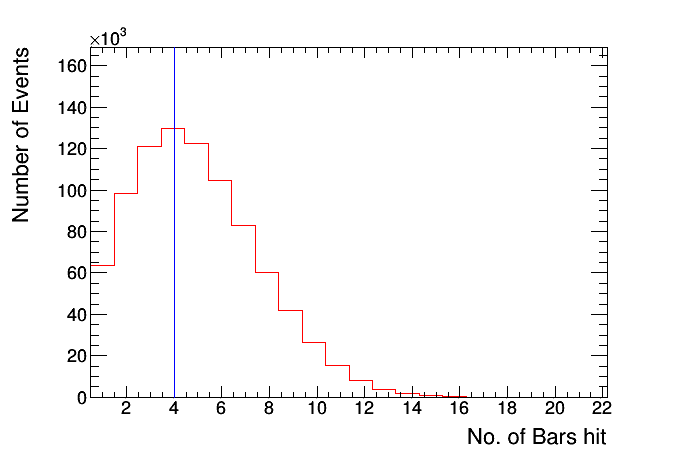
\includegraphics[width=\linewidth]{4n0_1MeVbars.png}
  \captionsetup{width=.9\linewidth}
  \caption{Number of bars hit by gadolinium cascade after absorbing neutrons of energies 25\,eV-75\,eV. With a bar cut of $\geq$ 4 giving 67.9\,\% acceptance.}
  \label{4bar_n_cut}
\end{subfigure}%
\begin{subfigure}{.5\textwidth}
  \centering
  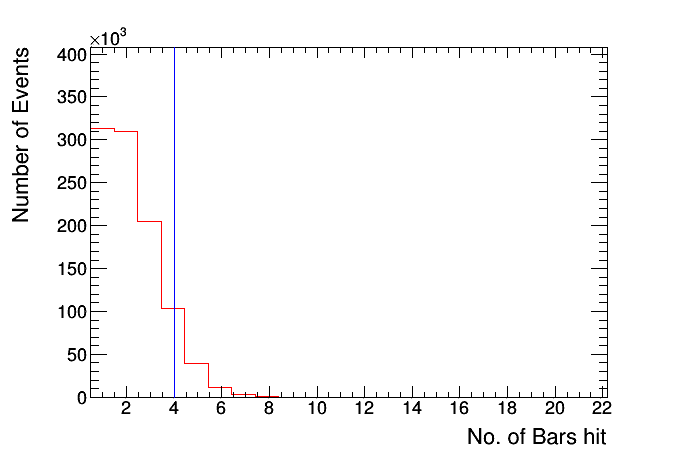
\includegraphics[width=\linewidth]{4e0_1MeVbars.png}
  \captionsetup{width=.9\linewidth}
  \caption{Number of bars hit from direct interactions of electrons of energies 0\,MeV-10\,MeV. With a bar cut of $\geq$ 4 giving 16.2\,\% acceptance. \\}
  \label{4bar_e_cut}
\end{subfigure}
\caption{Neutron and electron 4 bar cut on 2660 barred detector with a threshold of 0.1\,MeV.}
\label{4_bar_cut}
\end{figure}

\begin{figure}[H]
\centering
\begin{subfigure}{.5\textwidth}
  \centering
  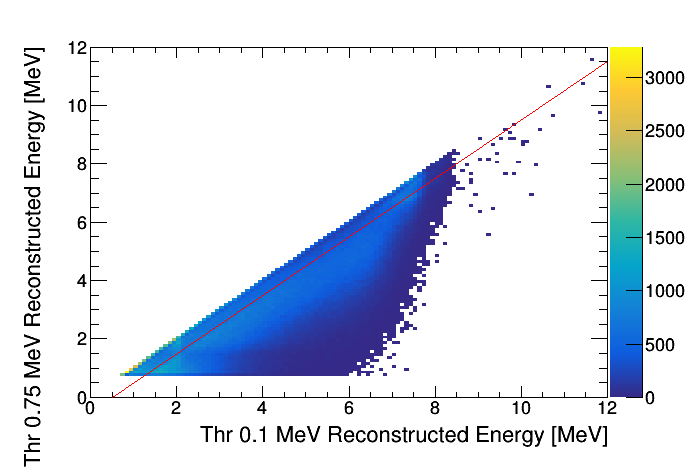
\includegraphics[width=\linewidth]{5n3000spread_recon_dual_thresh_0_1_0_75_line.png}
  \captionsetup{width=.9\linewidth}
  \caption{Reconstructed energies for thresholds 0.1\,MeV and 0.75\,MeV by gadolinium cascade after absorbing neutrons of energies 25\,eV-75\,eV. With a $E_\textrm{intercept}$ cut of 0.5\,MeV giving $\sim$ 70\,\% acceptance.}
  \label{2drecon_n_cut}
\end{subfigure}%
\begin{subfigure}{.5\textwidth}
  \centering
  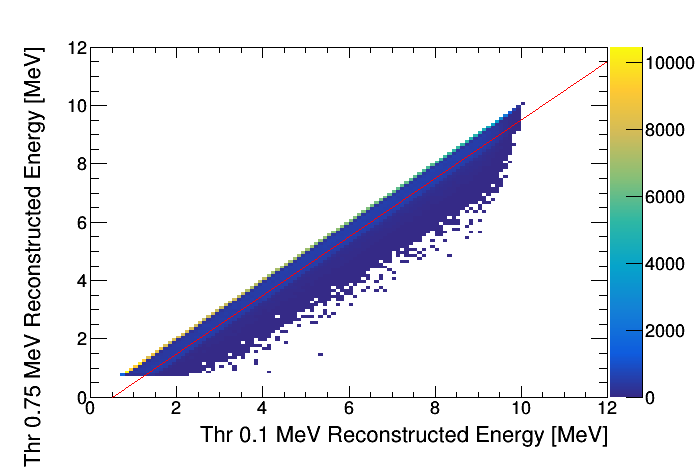
\includegraphics[width=\linewidth]{5e3000spread_recon_dual_thresh_0_1_0_75_line.png}
  \captionsetup{width=.9\linewidth}
  \caption{Reconstructed energies for thresholds 0.1\,MeV and 0.75\,MeV from direct interactions of electrons of energies 0\,MeV-10\,MeV. With a $E_\textrm{intercept}$ cut of 0.5\,MeV giving $\sim$ 17\,\% acceptance.}
  \label{2drecon_e_cut}
\end{subfigure}
\caption{0.1\,MeV Threshold and 0.75\,MeV Threshold reconstructed energy cuts for electrons and neutrons.}
\label{thr_thr_cut}
\end{figure}

More accurate cuts can be determined through measurements of the neutron acceptance and neutron to electron purity. The background for the purity is defined as a flat electron background with generated kinetic energies of 0\,MeV--10\,MeV, this is higher than expected but is used to demonstrate how to find the best cut. First, the preliminary cut in figure \ref{4_bar_cut} of 4 bars and then vary the threshold cut in figure \ref{thr_thr_cut} until we either have the highest purity or an acceptance $\geq$ 70\,\%. In figure \ref{purity_eff_full} we see the bar cut starting to dominate after a $E_\textrm{intercept}$ of 30\,pEq, there is very little reconstructed energy above 2\,MeV that also doesn't hit $\geq$ 4 bars. When $E_\textrm{intercept}$ is examined between 0-30 pEq as seen in figure \ref{purity_eff_zoom} the purity stabilises at 20 pEq and this gives us an acceptance of 74\,\%. This is within tolerance so our revised cuts are: 4 bars cut with a $E_\textrm{intercept}$ of 20\,pEq (0.8\,MeV). 

\begin{figure}[H]
\centering
\begin{subfigure}{.5\textwidth}
  \centering
  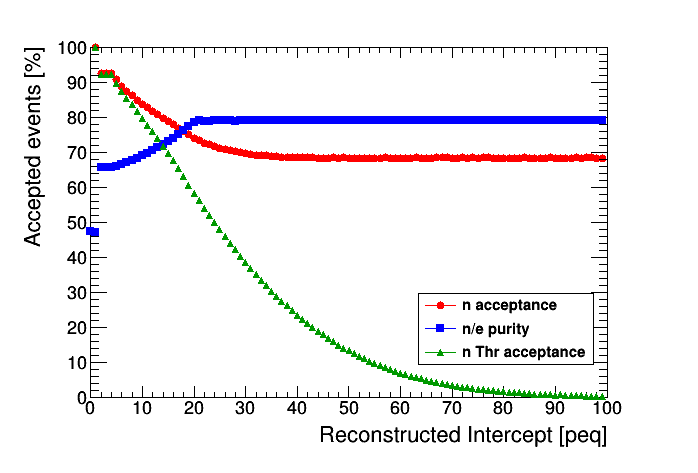
\includegraphics[width=\linewidth]{Trigger_efficency_and_purityne4.png}
  \captionsetup{width=.9\linewidth}
  \caption{neutron acceptance and purity for 4 bar cut over a $E_\textrm{intercept}$ of 0--100\,pEq. With acceptance of solo threshold cut for comparison.}
  \label{purity_eff_full}
\end{subfigure}%
\begin{subfigure}{.5\textwidth}
  \centering
  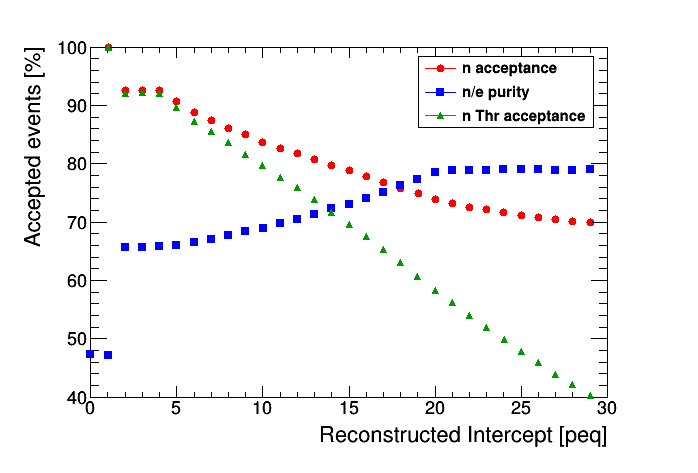
\includegraphics[width=\linewidth]{Best4barcut_ne.png}
  \captionsetup{width=.9\linewidth}
  \caption{neutron acceptance and purity for 4 bar cut over a $E_\textrm{intercept}$ of 0--30\,pEq. With acceptance of solo threshold cut for comparison.}
  \label{purity_eff_zoom}
\end{subfigure}
\caption{Purity and acceptance of the neutron signal over a $E_\textrm{intercept}$ of 0--100\,pEq and 0--30\,pEq. Errors on pEq of O $\sim$ $10^{-8}$\,pEq. Errors on acceptance of O $\sim$ $10^-3$\,\%.}
\label{purity_eff_both_cuts}
\end{figure}

Then when reconstructing the $e^-$ that pass through both cuts energies in MeV without smearing (figure \ref{sub_cuts_through_eng}) and in pEq with smearing (figure \ref{sub_cuts_through_png}) it is possible to determine the simulated noise. In figure \ref{cuts_through_eng_png} most events have an energy above 4\,MeV (100 pEq), electron noise with theses energies is unlikely. A more realistic noise function would mean fewer of these higher energy electrons are produced and so a more accurate cut that preserves more of the neutron signal would be possible in future. Only these rejection criteria are on the simulated neutron data presently, so the trigger acceptance percentage is equal to neutron efficiency percentage. Hence, neutron efficiency of the simulation is 74\,\% at present.  

\begin{figure}[H]
\centering
\begin{subfigure}{.5\textwidth}
  \centering
  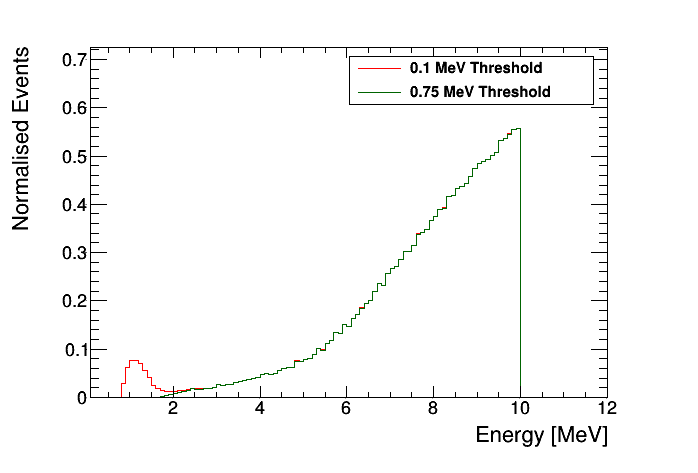
\includegraphics[width=\linewidth]{e_thresh_energy.png}
  \captionsetup{width=.9\linewidth}
  \caption{Generated kinetic electron energies passing both thresholds with cuts 4 bars and $E_\textrm{intercept}$ of 0.8\,MeV on threshold energies no smearing.}
  \label{sub_cuts_through_eng}
\end{subfigure}%
\begin{subfigure}{.5\textwidth}
  \centering
  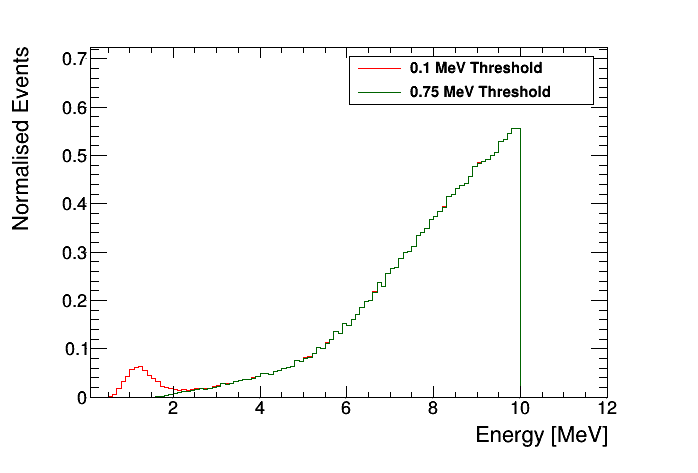
\includegraphics[width=\linewidth]{e_thresh_peq.png}
  \captionsetup{width=.9\linewidth}
  \caption{Generated kinetic electron energies passing both thresholds with cuts 4 bars and $E_\textrm{intercept}$ of 20\,pEq on threshold energies with smearing.}
  \label{sub_cuts_through_png}
\end{subfigure}
\caption{Generated energies of the e$^-$s for 2660 bar detector from both 0.1\,MeV and 0.75\,MeV bar thresholds without smearing \ref{sub_cuts_through_eng} and with smearing \ref{sub_cuts_through_png}.}
\label{cuts_through_eng_png}
\end{figure}

\subsection{Overall Anti-Neutrino Efficiency}
The overall anti neutrino detection efficiency can be calculated to first order by multiplying the $e^+$ and n efficiencies. The $\overline{\nu_e}$ efficiencies can be seen in table \ref{tab_3000_an_eff} for the 2660 barred detector. The efficiency for the positrons was determined via figure \ref{e+_3000_effs_thresh_0.1} for 2660 bars and \ref{e+_2000_effs_thresh_0.5} for 1862 bars. For the 2660 barred detector the efficiency and purity for the neutrons is determined by figure \ref{purity_eff_zoom} to be 73.9\,\% detector 78.6\,\% respectively with a requirement of 4 or more bars hit and a $E_\textrm{intercept}$ cut of 20\,pEq (0.8\,MeV). If we take the same cuts on the 1862 barred detector a neutron purity of 77.5\,\% is calculated with an efficiency of 69.4\,\% which allows table \ref{tab_2000_an_eff} to be constructed. \\ 
\begin{table*}[h]
\centering
\begin{tabular}{lllll}  
\toprule
\multicolumn{2}{c}{Positrons} & \multicolumn{1}{c}{Neutrons} & \multicolumn{1}{c}{Anti-neutrinos}
\\
\cmidrule(r){1-2}
\cmidrule(r){3-3}
\cmidrule(r){4-4}
Energy [MeV] & Efficiency [\%] & Efficiency [\%]  & Efficiency [\%]\\
\midrule
0-2          & 99.2            & 73.9             & 73.3\\
2-4          & 99.0            & ....             & 73.2\\
4-6          & 99.2            & ....             & 73.3\\
6-8          & 99.4            & ....             & 73.5\\
8-10         & 99.6            & ....             & 73.6\\
\bottomrule 
\end{tabular}
\caption{Efficiencies for 2660 barred detector for positrons neutrons and anti-neutrinos.}
\label{tab_3000_an_eff}
\end{table*}

\begin{table*}[h]
\centering
\begin{tabular}{lllll}  
\toprule
\multicolumn{2}{c}{Positrons} & \multicolumn{1}{c}{Neutrons} & \multicolumn{1}{c}{Anti-neutrinos}
\\
\cmidrule(r){1-2}
\cmidrule(r){3-3}
\cmidrule(r){4-4}
Energy [MeV] & Efficiency [\%] & Efficiency [\%]  & Efficiency [\%]\\
\midrule
0-2          & 99.1            & 69.4             & 68.8\\
2-4          & 98.9            & ....             & 68.6\\
4-6          & 99.1            & ....             & 68.8\\
6-8          & 99.3            & ....             & 68.9\\
8-10         & 99.5            & ....             & 69.1\\
\bottomrule  
\end{tabular}
\caption{Efficiencies for 1862 barred detector for positrons neutrons and anti-neutrinos. }
\label{tab_2000_an_eff}
\end{table*}

There is a improvement of $\sim$ 9.5\,\% $\overline{\nu_e}$\,\% efficiency between the original 1862 barred detector and the upgraded 2660 barred detector. Coupled with the improvement in contained energy as mentioned before in figure \ref{containment_comparison} this results in a significantly better signal for the upgraded detector, both in statistics and signal quality. This does not include the increase in statistics that the increase in mass will bring. $\sim$ 43\,\% more mass is being added to the detector which will boost the number of events recorded by $\sim$ 43\,\% if we combine these effects we get an overall increase of 43\,\% \times 1.095 $\approx$ 47\,\% in recorded events. With a better background function further improvement in the neutron efficiency is possible which will increase the $\overline{\nu_e}$\, efficiency in both cases.

%\section{Machine Learning approach }

\section{1st Year Conclusion and outlook}
\subsection{Summary}
In conclusion, these simulations indicate that the upgraded VIDARR detector will have an improvement on the anti-neutrino efficiencies of $\sim$ 47\,\%. Even with an unrealistically high level of background the proposed neutron trigger conditions of 4 bars hit and a $E_\textrm{intercept}$ of 20\,pEq on the thresholds, produces results with 78.6\,\% neutron purity and neutron efficiency of 73.9\,\%. $e^+$ efficiencies are mostly unchanged from the original 1862 barred detector. \\

The single bar Monte Carlo simulations allowed for a better understanding of cosmic muons interacting and stopping inside a bar, as well as demonstrating the effect that the TiO$_2$ coating can have even with low 20\,\% coating of TiO$_2$ (figures \ref{muon_pos_tio2_per} and \ref{proton_tio2_per}). \\

The Monte Carlo simulations of the full detector have proven useful in constraining the upper bound of the $e^+$ particle and energy reconstruction efficiencies (figures \ref{2000_p_sec} and \ref{3000_p_sec}). As well as constraining a lower bound for the neutron trigger and the neutron efficiency (at present equal to the neutron acceptance) and purity. These simulations have also allowed for an approximation of the statistical smearing (figure \ref{10phot_pois_gaus}) which shows that the Hydrogen peak could potentially be used for calibration purposes even when taking into account the counting statistics of the MPPCs (figure \ref{sub_3000_gd_h_peq}).

\subsection{Future Work}
Full testing of the Gadolinium models (figure \ref{evap_fnst_gd}) and the creation of a more accurate background noise function in the neutron events will need to be addressed. Whether editing one of the in built Gadolinium models or building a more detailed Gadolinum model from simulated data from the upgraded VIDARR itself is best will be determined once the electronics have been tested. The background noise function will at first have to be a rough approximation, such as using the $\gamma$s that are present in reactors, but it will be important for positrons as well if we are interested in observing the Compton edge of the annihilation $\gamma$s (figure \ref{Compton_edge_cuts_and_no_cuts}) as it may be unobservable with an appropriate noise function. \\

Further geometric effects need to be properly assessed a basic adjacency cut for the positrons has already been trialled with no noise, with some success but with has adverse effects on the energy reconstruction efficiency. A different approach to the geometric selection criteria (such as clustering) will improve the energy reconstruction. Furthermore tests with a neutron source would be trialled as sources with appropriate neutron energies are easier to obtain than $e^+$ sources with kinetic energies between 1-10\,MeV.\\

There may also be alternative methods to increasing statistics, it is possible that machine learning could be implemented at some point in the future. For example the reconstruction of partial events which can extrapolate from the geometry of events that are incomplete (edge events, particularly for neutrons) or too noisy, possibly extrapolating to improve containment as well. But it is possible that the simulated and/or measured data is not well suited to machine learning, or that the potential improvements it offers are not significant. 

%%%%%%% Everything from this point onwards has not been checked, so go over it later %%%%%%%
\section{Machine Learning approach} 
Machine learning has many different implementations that range in complexity, as computing power has increased so to has the capability to test more advanced machines. The most complex and well known of these would be the deep learning neural network [citation needed], a form of machine learning that utilities nodes in a simplified model of how human neurons work in the brain. Another well known and largely implemented form of machine learning is the support vector machine (SVM) \cite{kernelSVMs1992}, which uses statistical separation of the data points to draw a separating hyperplane between those points. Both of these compare favorably to boasted decision trees (BDTs) [citation needed] which can be quite limited in their approach to problem solving, this is because of their relative simplicity, they are easy to implement and understand but require careful application or a large number of dimensions to accurately solve problems.

\subsection{Support Vector Machine}
The SVM came to prominence in the early 1990s, an SVM with a polynomial kernel was used in 1992 to distinguish hand written characters \cite{kernelSVMs1992}. An SVM uses margins to determine the separation of certain data points whilst in the training phase. An SVM is comprised of support vectors that determine these margins and the separating hyperplane that is determined by the width of these margins \textbf{M$^*$} seen in figure \ref{svm_training}. The decision function, that the separating hyperplane represents is shown in equation \ref{hyperplane_Decision} where $\phi_{i}(\textbf{x})$ represents the feature sets of the data that is used for training and $w_i$ and $b$ are adjustable parameters of the SVM\cite{kernelSVMs1992}. The $\phi$ represents a predefined function of \textbf{x}, note that in figure \ref{svm_training} the decision function $D(\textbf{x})$ only uses a simplistic version of the SVM and so the decision boundary $D(\textbf{x})$ does not contain a $\phi$, it is $\textbf{w} \cdot \textbf{x} +b$. 

\begin{equation}
D(\textbf{x}) = \sum_{i=1}^{N} w_i \phi_{i}(\textbf{x}) + b 
\label{hyperplane_Decision}
\end{equation}

\begin{Figure}
 \centering
 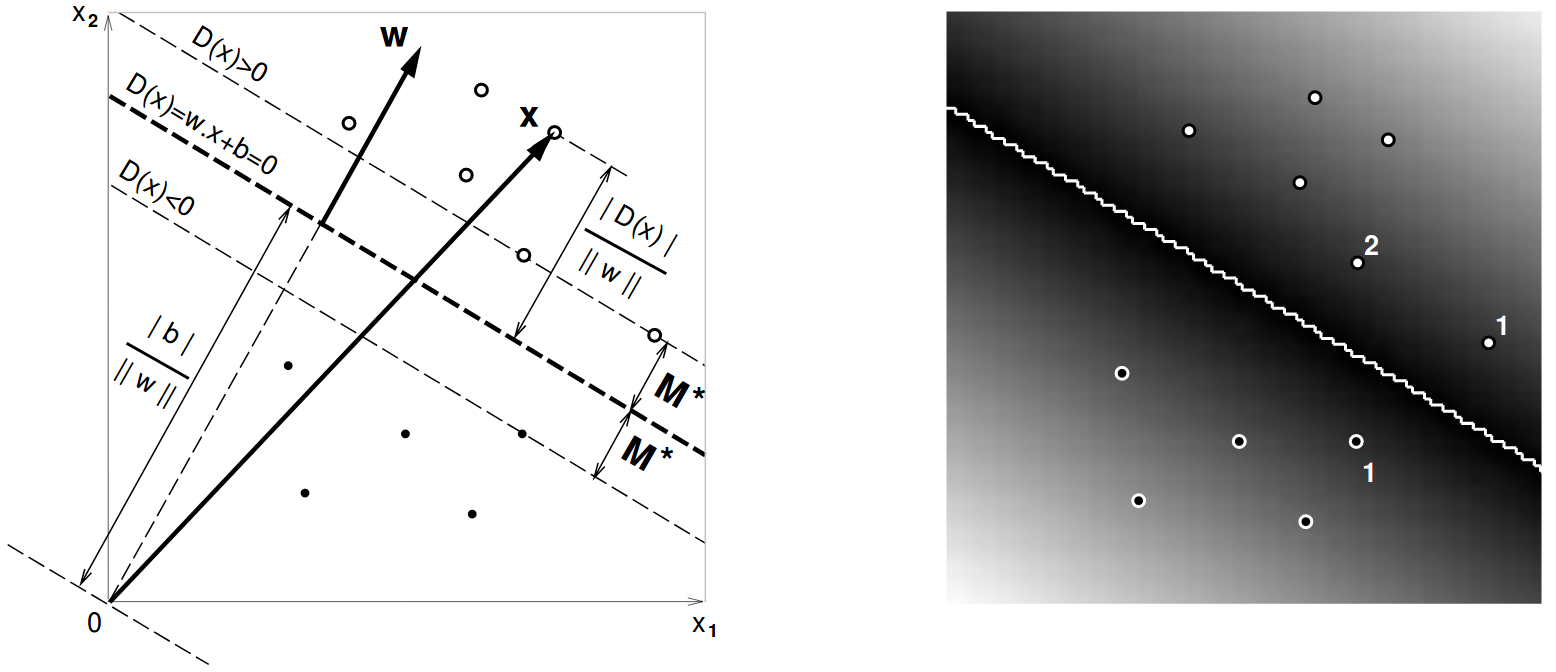
\includegraphics[height=71mm]{boserSVM_Training.png}
 \captionof{figure}{Training an SVM from \cite{kernelSVMs1992}.\\} %~can be used as a kind of place holder in latex
 \label{svm_training}
\end{Figure} 

In the training phase there are two classes that the SVM classifies against for A and B the condition is given by equation \ref{points} \cite{kernelSVMs1992}.
\begin{equation}
(\textbf{x}_1,y_1), (\textbf{x}_2,y_2), (\textbf{x}_3,y_3), ..., (\textbf{x}_p,y_p)
\label{points}
\end{equation}
\begin{center}
where $y_k$ = 1 if $x_k$ $\in$ class A\\ 
and   $y_k$ = -1 if $x_k$ $\in$ class B
\end{center} 
All the points on the positive support vector would be listed as $y_k = 1$, whereas all points on the negative support vector would be listed as $y_k = -1$. For an SVM with no kernel the $D(\textbf{x})  > 0$ gives a positive result and $D(\textbf{x})  < 0$ gives negative result as seen in figure \ref{svm_training}. For all samples that are positive they must give a result of 1 or greater, equation \ref{positive_data}, and vice versa for negative samples seen in equation \ref{negative_data}\cite{mitLecture}:
\begin{equation}
D(\textbf{x}) \geq \textbf{x$_+$} \cdot \textbf{w} + b \geq +1 
\label{positive_data}
\end{equation}
\begin{equation}
D(\textbf{x}) \leq \textbf{x$_-$} \cdot \textbf{w} + b \leq -1 
\label{negative_data}
\end{equation}
This is one of the key assertions of the support vector machine when training. Then using the mathematical convenience of $y_k$ it is possible to multiply the positive sample equation (equation \ref{positive_data}) by $y_k = +1$ and the negative sample equation (equation \ref{negative_data}) by $y_k = -1$ to get: 
\begin{equation}
y_k D(\textbf{x$_k$}) \geq y_k(\textbf{x$_k$} \cdot \textbf{w} + b) \geq +1 
\label{data_equation}
\end{equation}
Equation \ref{data_equation} describes all data that does not lie on the decision boundary and is greater than or equal to our margins \cite{mitLecture}. So by changing the equality in equation \ref{data_equation} to an = and subtract 1 equation \ref{support_vector_equation} is produced:
\begin{equation}
y_k D(\textbf{x$_k$}) -1 = y_k(\textbf{x$_k$} \cdot \textbf{w} + b) - 1 = 0
\label{support_vector_equation}
\end{equation}
This is now the support vector equation, it this condition that the SVM is trying to fulfill during its training phase \cite{mitLecture}.\\

The two primary constraints on the SVM during its training phase are now defined (equations \ref{hyperplane_Decision} and \ref{support_vector_equation}), now the width between the positive and the negative data sets is required is order to maximize the margin during the training phase as required \cite{kernelSVMs1992}. All training data points will satisfy the equation \ref{margin_condition} \cite{kernelSVMs1992}, in order to maximize the the margins to give $M^*$ equation \ref{maximise_width} is required \cite{kernelSVMs1992}. Finally this reduces to equation \ref{max_margin_condition} giving the maximum separation between the margins \textbf{w$^*$} \cite{kernelSVMs1992}.   

\begin{equation}
\frac{y_k D(\textbf{x$_k$})}{\mid\mid{\textbf{w}}\mid\mid} \geq M
\label{margin_condition}
\end{equation}
\begin{equation}
\underset{k}{\textnormal{min}} ~  y_k D(\textbf{x$_k$}) = M^*
\label{maximise_width}
\end{equation}
\begin{equation}
\underset{\textbf{w}}{\textnormal{min}} \mid\mid \textbf{w} \mid\mid ^2
\label{max_margin_condition}
\end{equation}

The problem in equation \ref{max_margin_condition} can be solved by transforming it into dual space by the use of a Largrangian \cite{kernelSVMs1992}, \cite{svm_book} seen in equation \ref{lagrange_solver}.
\begin{equation}
L (\textbf{w},b,\alpha) = \frac{1}{2} \mid\mid \textbf{w} \mid\mid ^2 - \sum_{k=1}^{P} \alpha_k [y_kD(\textbf{x$_k$}))-1]
\label{lagrange_solver}
\end{equation}
The SVM wants to maximize the margin, this corresponds to minimizing the \textbf{w} value as equations \ref{maximise_width} and \ref{max_margin_condition} show \cite{kernelSVMs1992}, \cite{mitLecture}, \cite{svm_book}. Substituting in $D(\textbf{x$_k$}) = \textbf{x$_k$} \cdot \textbf{w} + b$ into equation \ref{lagrange_solver} and then differentiating to find the minimum with respect to \textbf{w} gives a value for the minimal \textbf{w} (\textbf{w$^*$}) seen in equation \ref{minimum_W} \cite{kernelSVMs1992}, \cite{mitLecture}.
\begin{equation}
\textbf{w}^* = \sum_{k=1}^{P} \alpha^*_k y_k \phi_k
\label{minimum_W}
\end{equation}
Note again that $\phi_k$ is a feature set of \textbf{x} so this can be replaced to give a simplified version of the equation seen in \ref{simplfied_min_w} \cite{mitLecture},\cite{svm_book}.
\begin{equation}
\textbf{w}^* = \sum_{k=1}^{P} \alpha^*_k y_k \textbf{x$_k$}
\label{simplfied_min_w}
\end{equation}
The Lagrangian must also be differentiated with respect to b, as b is also a variable that can vary the Lagrangian, when rearranged this gives equation \ref{simplified_max_b} \cite{mitLecture} ,\cite{svm_book}.
\begin{equation}
- \frac {\partial{L}}{\partial{b}} = \sum_{k=1}^{P} \alpha^*_k y_k = 0 
\label{simplified_max_b}
\end{equation}
By substituting the equations \ref{simplfied_min_w} and \ref{simplified_max_b} into equation \ref{lagrange_solver} we get the result described by equation \ref{lagrange_solver_compleate} \cite{mitLecture}, \cite{svm_book}.
\begin{equation} 
L (\textbf{w},b,\alpha) = \sum_{k=1}^{P} \alpha^*_k - \frac{1}{2}  \sum_{k=1}^{P} \sum_{l=1}^{P} \alpha^*_k \alpha^*_l y_k y_l  \textbf{x$_k$} \cdot \textbf{x$_l$}
\label{lagrange_solver_compleate}
\end{equation}
This allows us to see finally see the Lagrangian solution for the SVM in dual space, this is a convexly optimized problem \cite{mitLecture}, \cite{svm_book}. This means that there is only one global minimum in the whole data set, as a result there is no chance of getting stuck on local minima seen in other forms of machine learning. However equation \ref{lagrange_solver_compleate} also shows a weakness of the SVM, the problem is a quadratic equation relying on both the values for k and l in a given vector space. This limitation means that for a given number of data points n n$^2$ computations are required for optimization, which is computationally expensive. Further all of the feature sets are required in order to optimize effectively. However these problems can be somewhat overcome with the application of the Sequential Minimal Optimization developed by Microsoft in 1998 \cite{microsoft_smo}. 

\subsubsection{Kernel SVM}
The above solution only works for a purely linear SVM, however in reality problems may not be linearly separable in which case a kernel SVM is required. A kernel SVM uses a kernel to transform a non-linear problem into a linear problem by transforming the data in the input space by using the inner product. This allows for SVMs to have access to a low-dimensional input space instead of the high-dimensional feature space, thus helping to prevent over-fitting. \cite{svm_book}. The mapping for the Kernel does not need to be explicitly known \cite{svm_book}. The Kernel is a function of the x values, and so can be substituted into the decision function (equation \ref{hyperplane_Decision}) and the Lagrange equation \ref{lagrange_solver_compleate} by imputing $K(\textbf{x}_i,\textbf{x}_j)$ instead of $(\textbf{x}i,\textbf{x}j)$ \cite{kernelSVMs1992}, \cite{mitLecture}. %This explanation is a bit iffy    

\begin{Figure}
 \centering
 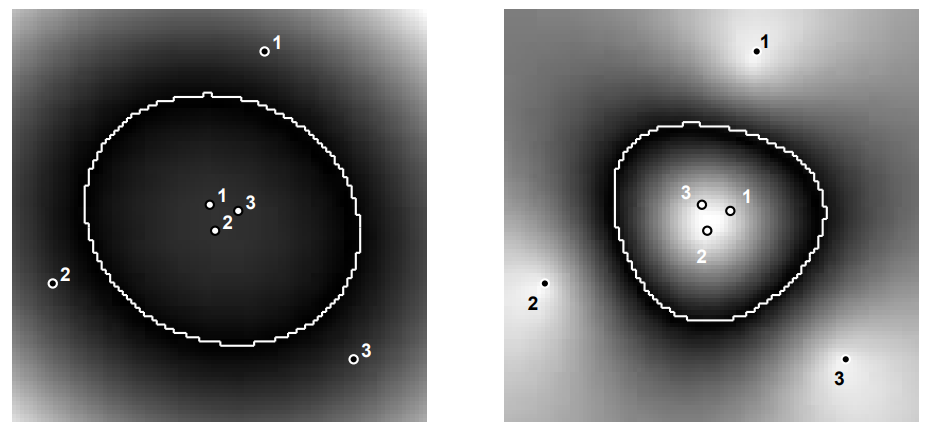
\includegraphics[height=71mm]{Kernel_svm_examples_boser.png}
 \captionof{figure}{The use of differing Kernels on linearly non-seperatble data with $K(\textbf{x},\textbf{x'}) = (\textbf{x} \cdot \textbf{x'} + 1)^2$ (left) and an exponential RBF $K(\textbf{x},\textbf{x'}) = \exp{(-\mid \mid \textbf{x} - \textbf{x'} \mid \mid/2)}$ (right) from \cite{kernelSVMs1992}.\\} %~can be used as a kind of place holder in latex
 \label{svm_kernels}
\end{Figure} 

The kernels used in the software package LIBSVM \cite{libsvm_paper} can be seen in equations \ref{linear_K_equation} - \ref{sigmoid_K_equation}. The linear kernel \ref{linear_K_equation} is used for data that is linearly separable, it has minimal impact on how the SVM operates. The polynomial kernel, equation \ref{poly_K_equation}, is a flexible kernel that can approximate a linear data-set if required if the coefficient r is 0, $\gamma$ = 1 with degree d also = 1. But can also uses these parameters to eventually fit any data-set lienar or non-linear. The radial basis function (RBF) kernel, equation \ref{rbf_K_equation}, transforms the data using a Gaussian like function, which allows for non linear solutions to be found, it has fewer free parameters than the polynomial kernel. However this kernel can struggle with linear data-sets and a larger range of $\gamma$s than the polynomial kernel may be required in order to get the most accurate answer. The sigmoid kernel was not used as the problems encountered were not easy to solve by use of a hyperbolic tangent function. The ideal kernels for seperating data for VIDARR were the polynomial and RBF kernels.  

\begin{equation}
K_{Linear}(\textbf{x},\textbf{x'})= (\textbf{x},\textbf{x'})
\label{linear_K_equation}
\end{equation}
\begin{equation}
K_{Poly}(\textbf{x},\textbf{x'}) =  (\gamma(\textbf{x},\textbf{x'})+r)^d 
\label{poly_K_equation}
\end{equation}
\begin{equation}
K_{RBF}(\textbf{x},\textbf{x'}) =  \exp{(-\gamma \mid \mid \textbf{x} - \textbf{x'}  \mid \mid ^2)}
\label{rbf_K_equation}
\end{equation}
\begin{equation}
K_{Sigmoid}(\textbf{x},\textbf{x'}) =  \tanh{(\gamma(\textbf{x},\textbf{x'})+ r)} 
\label{sigmoid_K_equation}
\end{equation}

\subsubsection{LIBSVM and LIBLINEAR}
LIBSVM and LIBLINEAR are libraries developed by the national University of Taiwan \cite{libsvm_paper}, \cite{liblinear_paper}. They are frequently used libraries that are widely used enough to be partially credited for the SVM's success \cite{svm_book}, they come with different advantages. \\

LIBSVM can fit data linearly or with a kernel using two parameters C and $\gamma$. C is necessary for the SVM regardless of Kernel as it determines the aggressiveness of the margins, with C = 1 being the standard, C = 0.1 being less aggressive (softer) and C = 10 being more aggressive (harder). In terms of physical data this corresponds generally to higher efficiency with a soft margin and higher purity with a harder margin. The softer margin allows for more miss classifications to be made, but is more general, and vice versa. The variable $\gamma$ is for the kernel it determines the variations between differing points in the data set, allowing for greater discrepancies to be made, with $1/n$ being the standard. LIBSVM's problem however is that its SMO is not optimized for data sets $>$ $10^5$ as the data sets in the Monte Carlo simulations can exceed $10^6$ we have to make use of the other library. \\

LIBLINEAR is a program that is designed for the application of big data classification capable of handling at least $10^6$ \cite{liblinear_paper} and can train on even larger data sets. When testing this library it was possible to train the data set up to $10^7$ data points within a reasonable time. Our simulations simulate $10^6$ signal events and $10^6$ noise events, the signal of IBD are e$^+$s and neutrons, the noise is typically comprised of $\gamma$s and e$^-$s. Cosmic $\mu$s are also a key source of noise however basic tracking can exclude them. This puts the number of data sets at \sim ~4$\times 10^6$ without Cosmic events and \sim ~5$\times 10^6$ with Cosmic events. This library is suitable for our purposes, however LIBLINEAR does not come with a kernel implementation. This either requires the use of kernel being implemented directly or being approximated. \\

Kernels however also suffer from  a similar memory issue as SVMs. However the kernel memory issues scales with n$^3$ \cite{nystrom_paper} instead of n$^2$ seen in the SVM \cite{microsoft_smo} where n is the number of training samples. But by taking random samples of number m of the data sets in question the problem scales with m$^2$n, this causes a significant improvement in the speed of the kernel SVM. This kernel approximation was used with LIBLINEAR to work on large simulated data sets for the trigger data. 

\subsection{Application to Trigger Data}
The trigger data in section \ref{trigger_section_by_hand} is a data set with 4 features: reconstructed energy at a threshold of 0.1\,MeV, reconstructed energy at a threshold of 0.75\,MeV, \# of bars hit at a threshold of 0.1\,MeV and \# of bars hit at a threshold of 0.75\,MeV. This data can then be fed to an SVM in order to find the best separation between the data points of signal (neutrons) and noise (electrons). SVMs are multidimensional, able to work with a large number of features, but more than 3 dimensions can be hard to visualize. Figure \ref{SVM_examples} shows a 2D representation of how the SVM separates these data sets for reconstructed energy \ref{sub_SVM_examples_recon} and bars \ref{sub_SVM_examples_bars}. Interestingly the SVM was able to find a bar cut that was better than the proposed 1D cut in section \ref{trigger_section_by_hand}, whereas the reconstructed energy cut is quite similar. 

\begin{figure}[H]
\centering
\begin{subfigure}{.5\textwidth}
  \centering
  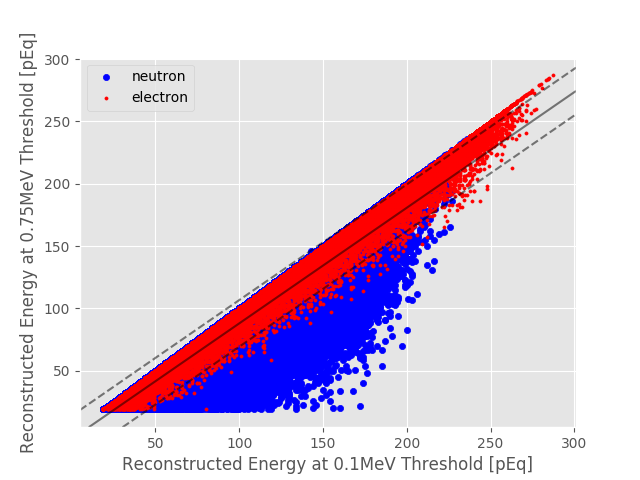
\includegraphics[width=\linewidth]{recon_0_1_vs_recon_0_75.png}
  \captionsetup{width=.9\linewidth}
  \caption{Reconstructed energy for neutrons and electrons at thresholds of 0.1\,Mev and 0.75\,MeV with an SVM separating them.}
  \label{sub_SVM_examples_recon}
\end{subfigure}%
\begin{subfigure}{.5\textwidth}
  \centering
  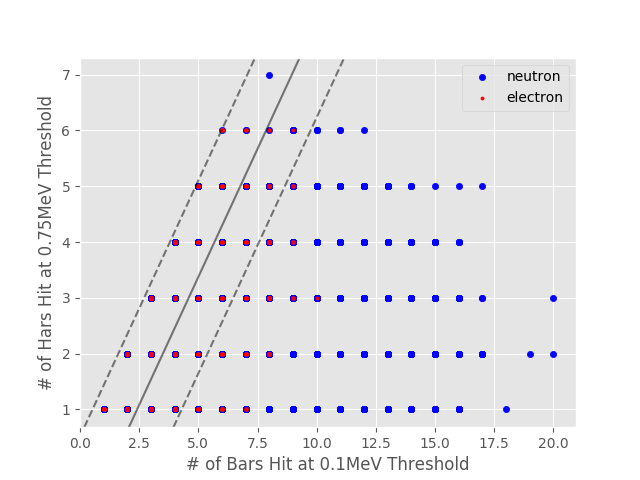
\includegraphics[width=\linewidth]{bars_0_1_vs_bars_0_75.png}
  \captionsetup{width=.9\linewidth}
  \caption{Number of bars hit for neutrons and electrons at thresholds of 0.1\,Mev and 0.75\,MeV with an SVM separating them.}
  \label{sub_SVM_examples_bars}
\end{subfigure}
\caption{How an SVM separates the data points for different variables, depending on reconstructed energy or number of bars hit}
\label{SVM_examples}
\end{figure}

A key component of measuring a classifiers effectiveness is accuracy, which is defined as the number of events that are correctly measured over the total number of events $\times$ 100. The accuracy of \ref{sub_SVM_examples_recon} is $\sim$  80.5\,\% $\sim$ 85\,\%. However \ref{sub_SVM_examples_recon} only represents two features as does \ref{sub_SVM_examples_bars}, there are 4 features that may have up to 4 choices. That is 4C1 will have 4 different classifiers, 4C2 will have 6 different classifiers, 4C3 will have 4 classifiers and 4C4 will have 1 classifier. The accuracy for these differing classifier combinations for a linear SVM with a nystrom approximation can be seen in figure \ref{accuracy_of_lin_SVMs}. In figure \ref{accuracy_of_lin_SVMs} the accuracy of the classifier stabilizes at a choice of 2 features, when the best combination of E (reconstructed) at 0.1\,MeV threshold and \# of bars hit at 0.1\,MeV threshold are chosen.\\ 

However in addition to the accuracy of the classifier shown in figure \ref{accuracy_of_lin_SVMs} the efficiency and purity can also be measured to produce their own respective graphs. The neutron efficiency for each classifier can be seen in figure \ref{efficiency_of_lin_SVMs} and the neutron purity for each classifier can be seen in figure \ref{purity_of_lin_SVMs} the best classifier is the same in each case: E (reconstructed) at 0.1\,MeV threshold and \# of bars hit at 0.1\,MeV threshold. Giving an efficiency of 80\,\% and purity of 91\,\% for that classifier. When compared with the results in section \ref{trigger_section_by_hand} these results give a 6\,\% improvement in neutron efficiency of the proposed trigger and 11\,\% in the neutron purity of the proposed trigger whilst using 2 features instead of the 3 used in section \ref{trigger_section_by_hand}. When using this SVM classifier on the data set used in section \ref{trigger_section_by_hand} the figures \ref{svm_neutron} and \ref{svm_electron} are produced. 

\begin{Figure}
 \centering
 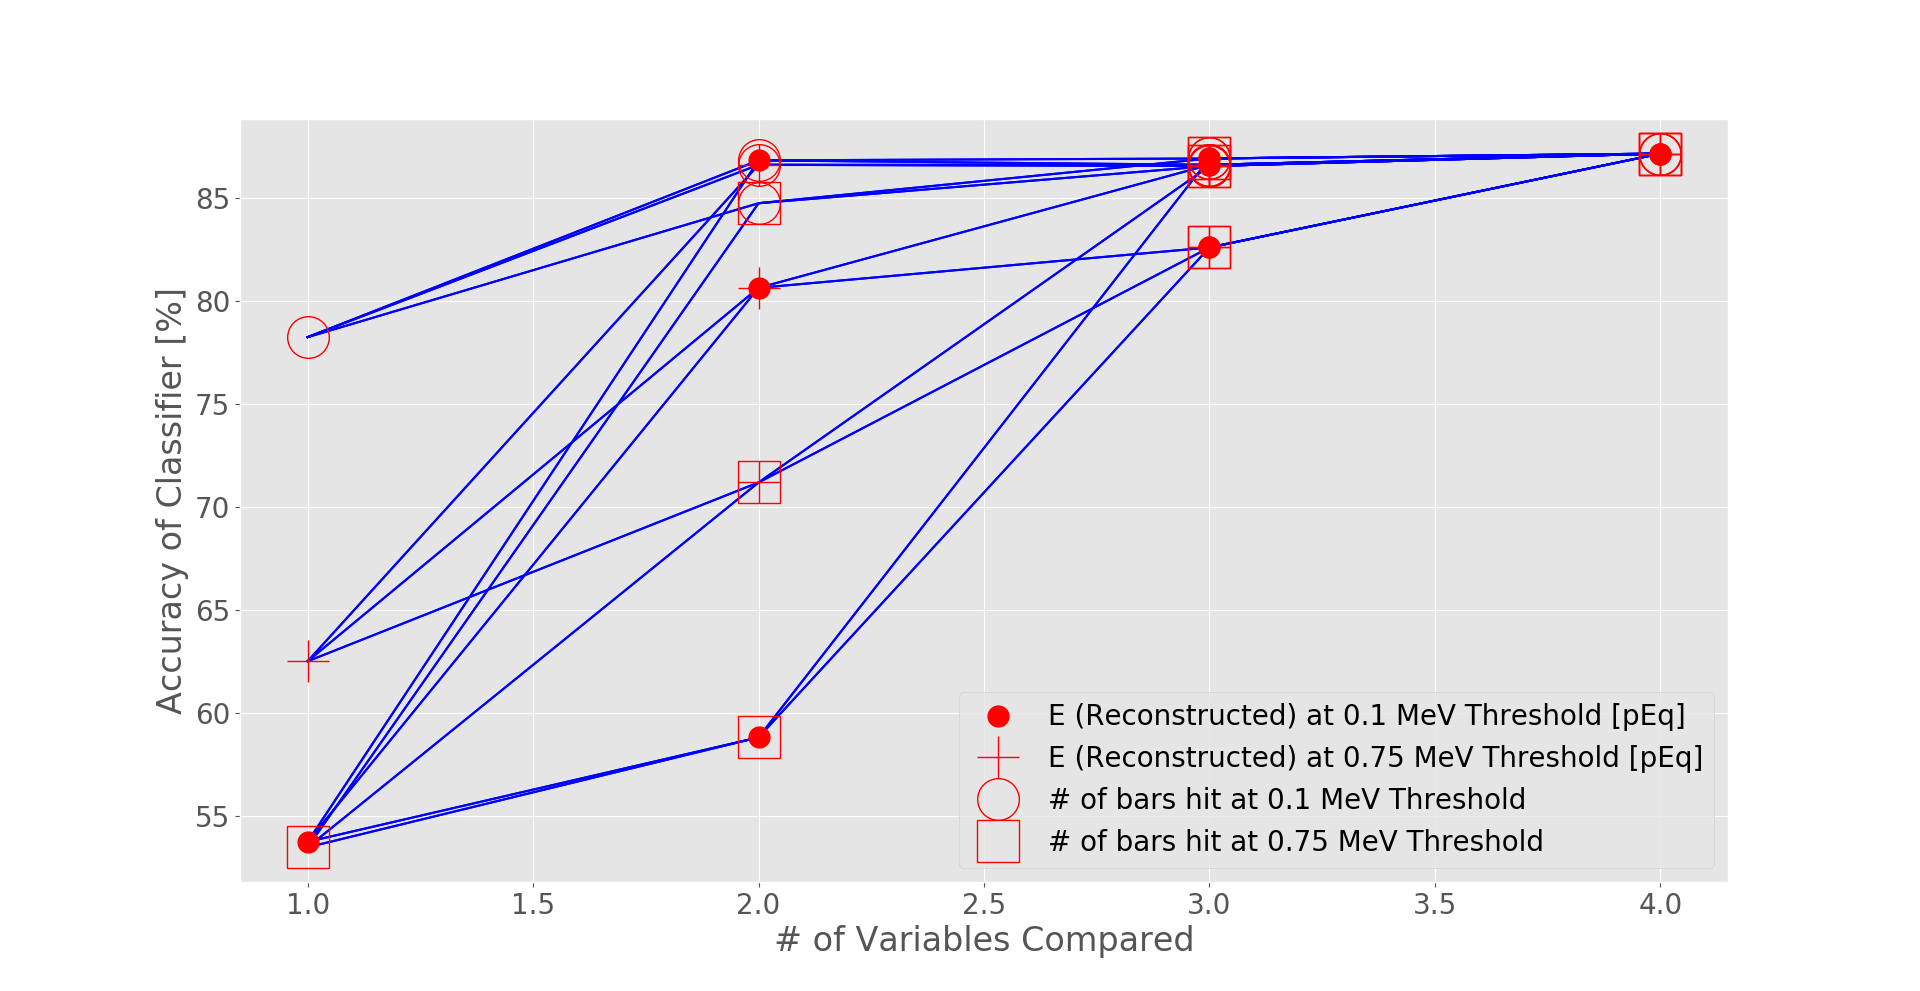
\includegraphics[height=100mm]{Accuracy_lin_SVM.png}
 \captionof{figure}{The accuracy of the SVM classifier as different variables are added to the classification, the best combination is E(Reconstructed) at 0.1\,MeV and \# of bars hit at 0.1\, MeV.} %~can be used as a kind of place holder in latex
 \label{accuracy_of_lin_SVMs}
\end{Figure} 

\begin{Figure}
 \centering
 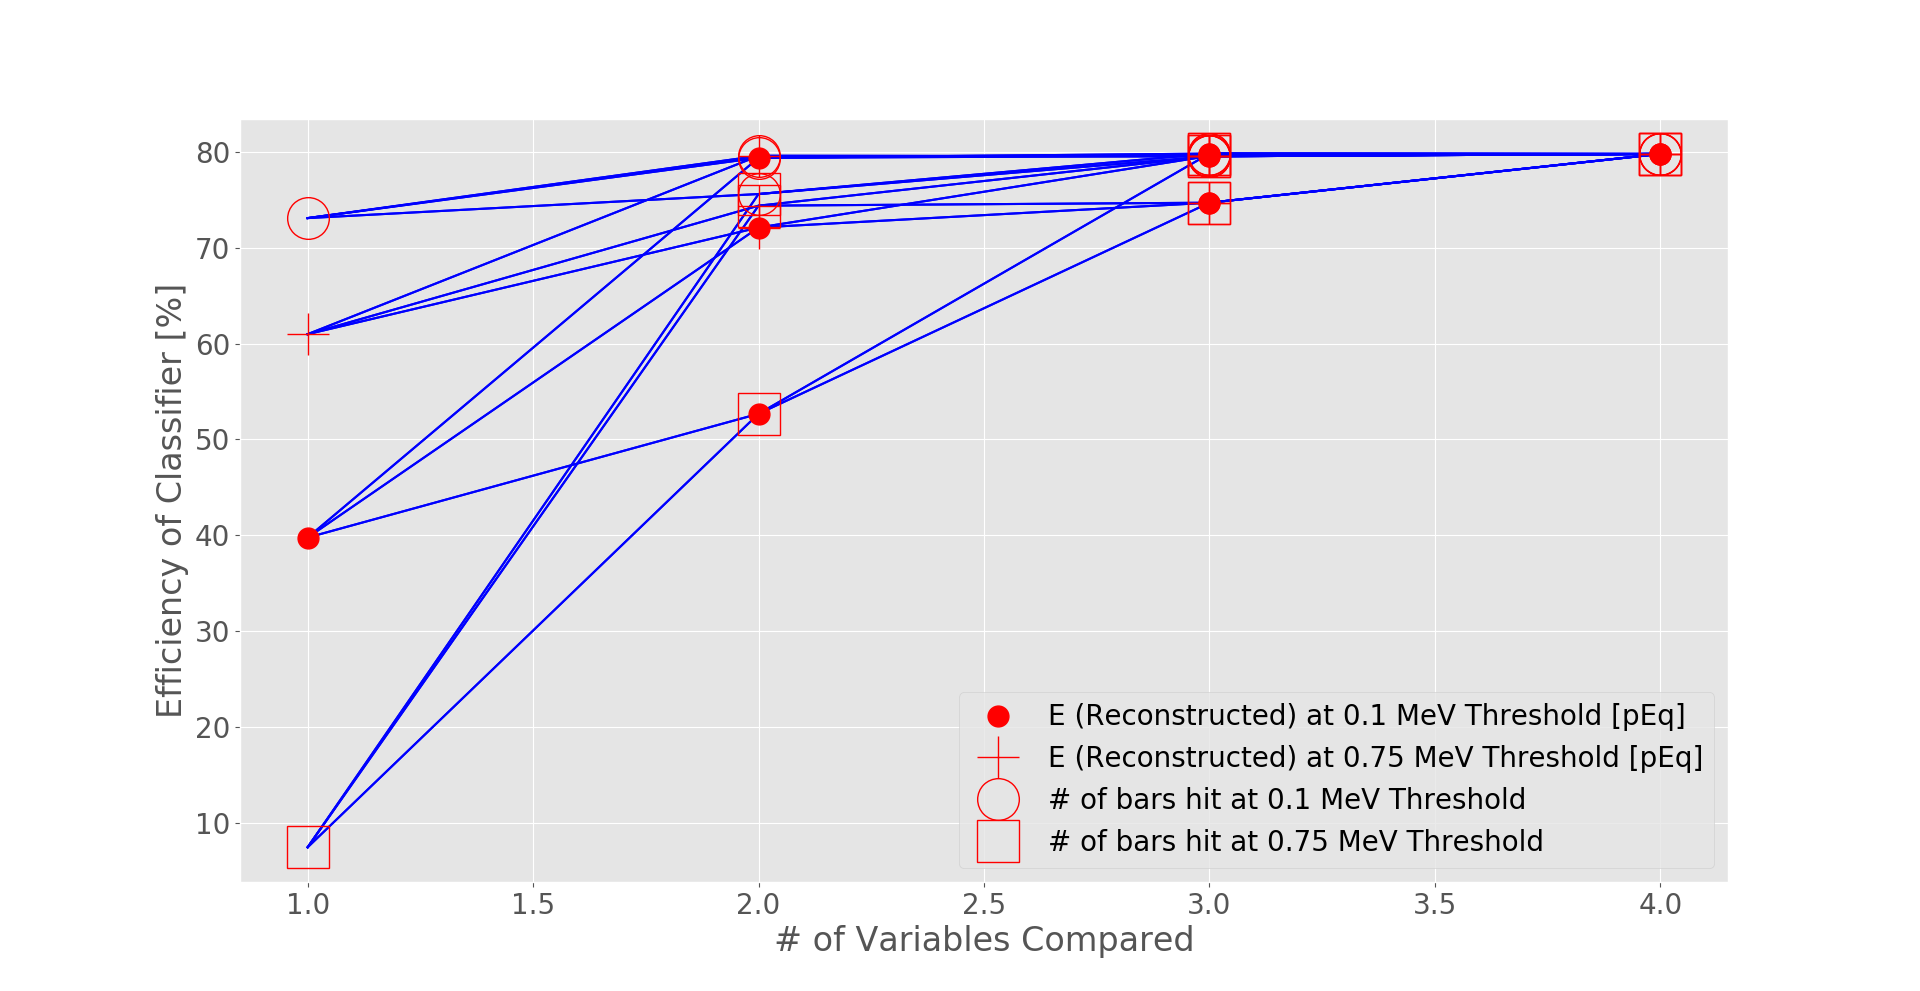
\includegraphics[height=100mm]{Efficency_lin_SVM.png}
 \captionof{figure}{The neutron efficiency of the SVM classifier as different variables are added to the classification, the best combination is E(Reconstructed) at 0.1\,MeV and \# of bars hit at 0.1\, MeV.} %~can be used as a kind of place holder in latex
 \label{efficiency_of_lin_SVMs}
\end{Figure} 

\begin{Figure}
 \centering
 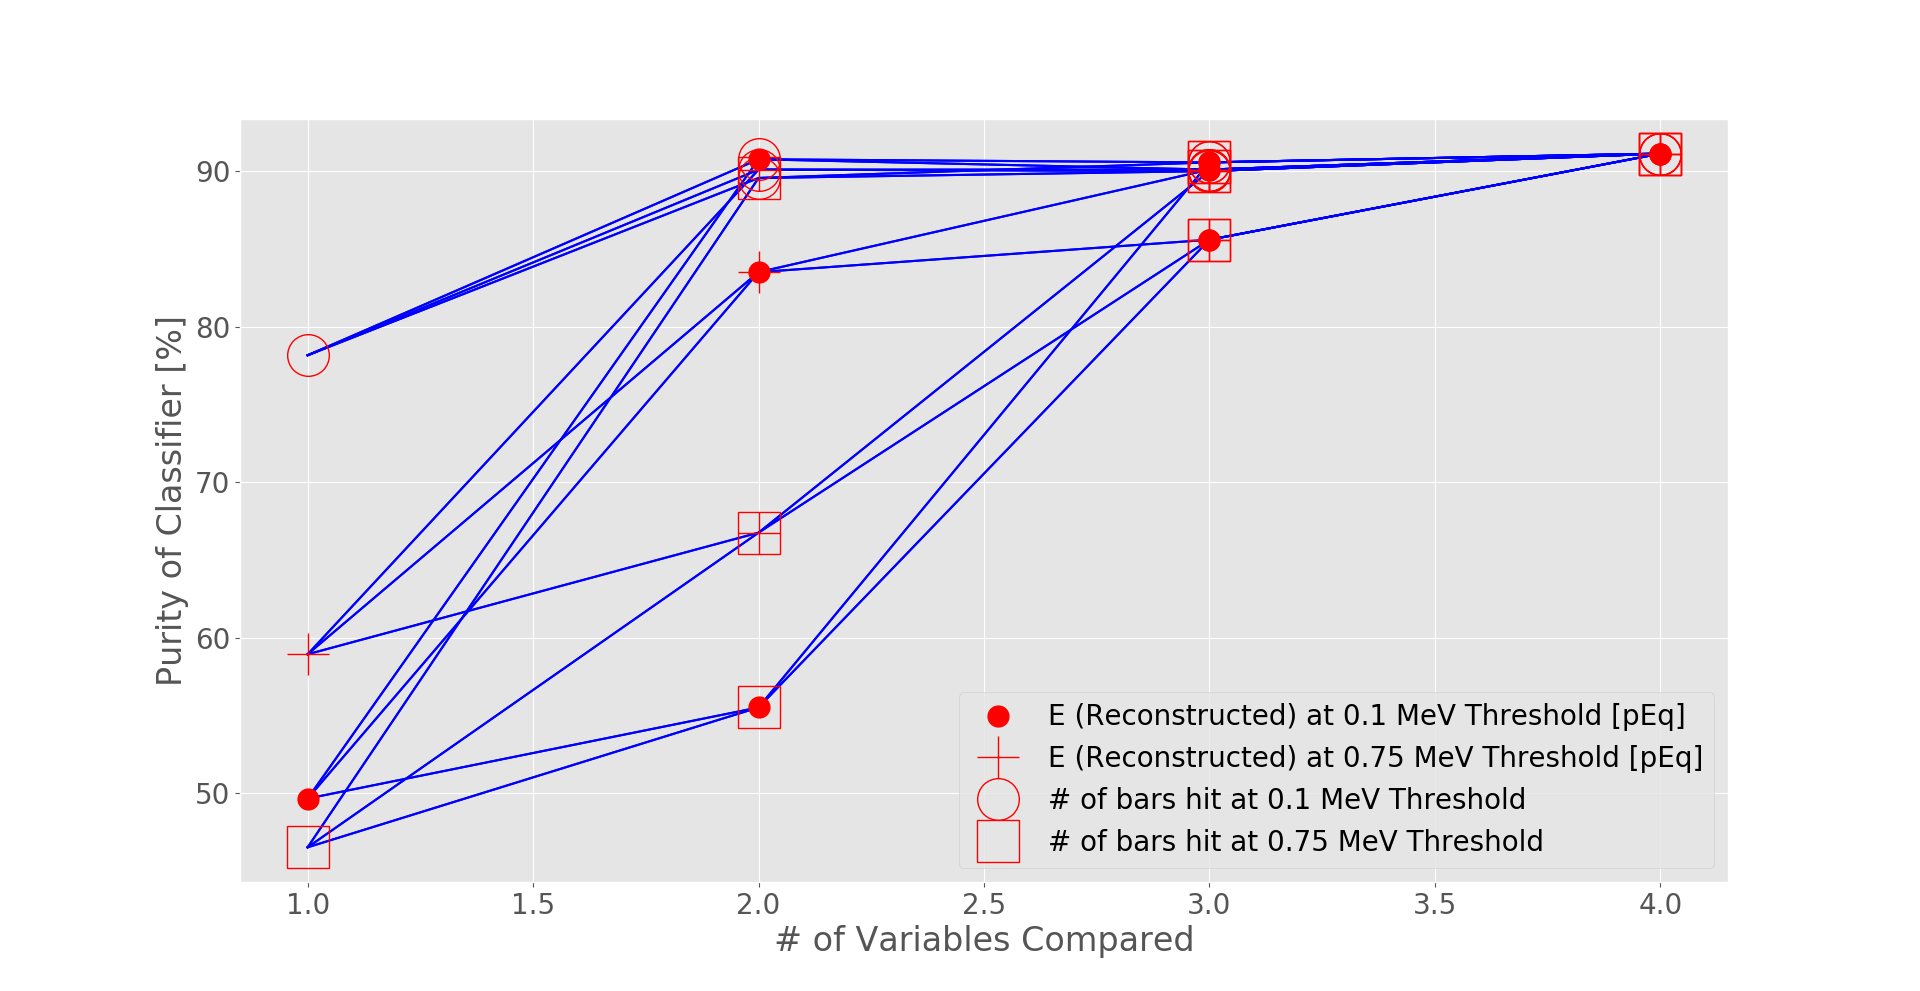
\includegraphics[height=100mm]{Purity_lin_SVM.png}
 \captionof{figure}{The neutron purity of the SVM classifier as different variables are added to the classification, the best combination is E(Reconstructed) at 0.1\,MeV and \# of bars hit at 0.1\, MeV.} %~can be used as a kind of place holder in latex
 \label{purity_of_lin_SVMs}
\end{Figure}

\begin{figure}[H]
\centering
\begin{subfigure}{.5\textwidth}
  \centering
  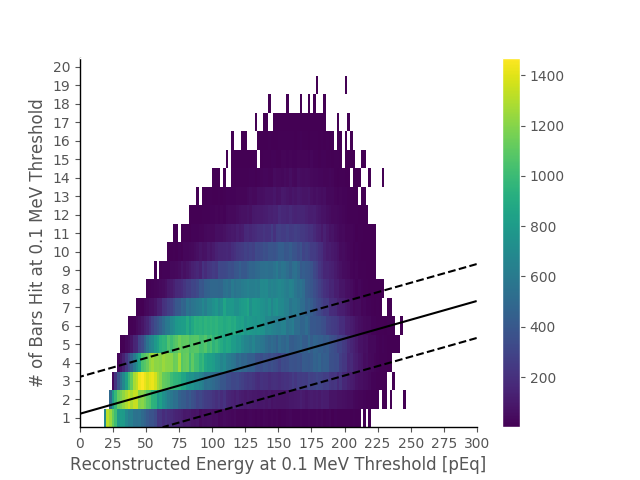
\includegraphics[width=\linewidth]{chosen_svm_neutron.png}
  \captionsetup{width=.9\linewidth}
  \caption{E(Reconstructed) at 0.1\,MeV and \# of bars hit at 0.1\,MeV for neutrons with the chosen trigger SVM shown.}
  \label{svm_neutron}
\end{subfigure}%
\begin{subfigure}{.5\textwidth}
  \centering
  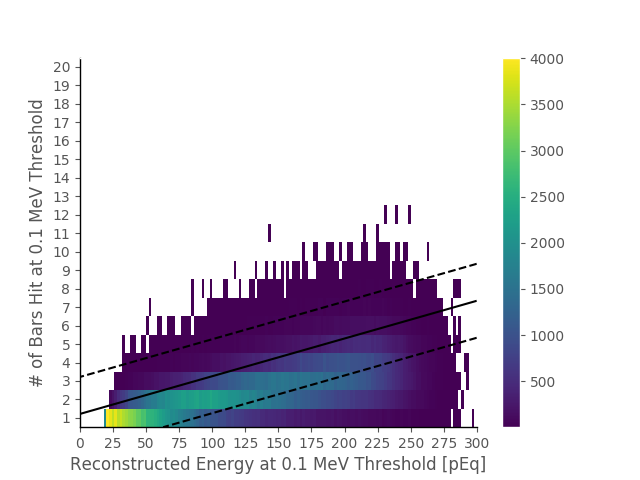
\includegraphics[width=\linewidth]{chosen_svm_electron.png}
  \captionsetup{width=.9\linewidth}
  \caption{E(Reconstructed) at 0.1\,MeV and \# of bars hit at 0.1\,MeV for electrons with the chosen trigger SVM shown.}
  \label{svm_electron}
\end{subfigure}
\caption{E(Reconstructed) at 0.1\,MeV and \# of bars hit at 0.1\,MeV for neutrons and electrons with the SVM seperating the neutron and the electron events. All hits above the line is classified as a neutron and all events below the line are classified as an electron in both \ref{svm_neutron}, \ref{svm_electron}. The margins represented by the dashed lines are wide due to the large spread of the neutron data. C=$10^6$}
\label{svm_on_neutrons_and_electrons}
\end{figure}

There are two values to tune the SVM, the hardness of the margins denoted often as C and the step required by a kernel in order to reach the global maximum often denoted as $\gamma$. Though $\gamma$ is only required for polynomial, sigmoid and radial base function (RBF) kernels, and so does not apply to figure \ref{svm_on_neutrons_and_electrons} as it is a linear SVM. The margin parameter C is considered hard $>$ 1 and soft $<$ 1 and default = 1. Soft margins give an SVM with a more generalized shape of the data, whereas a hard margin gives a more specific shape of the data with an increased risk of over-fitting. Both C and $\gamma$ vary from data-set to data-set in this case, figure \ref{svm_on_neutrons_and_electrons}, the margins were increased from $10^{-6}, 10^{-5}, ..., 10^6$ until the accuracy decreased. However in figure \ref{svm_on_neutrons_and_electrons} a decline in accuracy was never observed so the value of C = $10^6$.\\

Though the trigger cut is designed for an FBGA board and so must be linear it is possible to test a kernel SVM on the data sets used in order to observe the effects of different kernels on the same data-set. $\gamma$ was varied from $10^{-6}, 10^{-5}, ..., 10^6$ as was C, from this we were able to produce a polynomial kernel with $\gamma$ = 1 and C = $10^6$ with an accuracy of $\sim$ 86\,\%, seen in figure \ref{poly_svm_on_neutrons_and_electrons}. And then the process was repeated with an RBF kernel with $\gamma$ = 0.01 and C = 0.001 giving an accuracy of $\sim$ 86\,\% seen in figure \ref{rbf_svm_on_neutrons_and_electrons}.

\begin{figure}[H]
\centering
\begin{subfigure}{.5\textwidth}
  \centering
  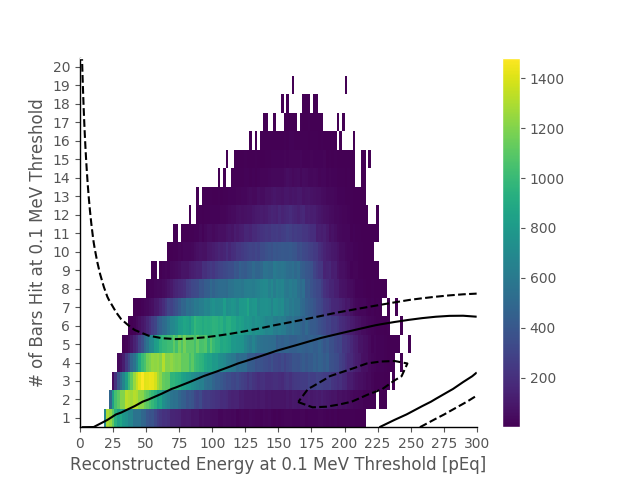
\includegraphics[width=\linewidth]{chosen_svm_neutron_poly.png}
  \captionsetup{width=.9\linewidth}
  \caption{E(Reconstructed) at 0.1\,MeV and \# of bars hit at 0.1\,MeV for neutrons with a polynomial kernel SVM shown.}
  \label{poly_svm_neutron}
\end{subfigure}%
\begin{subfigure}{.5\textwidth}
  \centering
  \includegraphics[width=\linewidth]{chosen_svm_electron_poly.png}
  \captionsetup{width=.9\linewidth}
  \caption{E(Reconstructed) at 0.1\,MeV and \# of bars hit at 0.1\,MeV for electrons with a polynomial kernel SVM shown.}
  \label{poly_svm_electron}
\end{subfigure}
\caption{E(Reconstructed) at 0.1\,MeV and \# of bars hit at 0.1\,MeV for neutrons and electrons with a polynomial kernel SVM seperating the neutron and the electron events.$\gamma$ = 1 and C = $10^6$. }
\label{poly_svm_on_neutrons_and_electrons}
\end{figure}

\begin{figure}[H]
\centering
\begin{subfigure}{.5\textwidth}
  \centering
  \includegraphics[width=\linewidth]{chosen_svm_neutron_rbf.png}
  \captionsetup{width=.9\linewidth}
  \caption{E(Reconstructed) at 0.1\,MeV and \# of bars hit at 0.1\,MeV for neutrons with an RBF kernel SVM shown.}
  \label{rbf_svm_neutron}
\end{subfigure}%
\begin{subfigure}{.5\textwidth}
  \centering
  \includegraphics[width=\linewidth]{chosen_svm_electron_rbf.png}
  \captionsetup{width=.9\linewidth}
  \caption{E(Reconstructed) at 0.1\,MeV and \# of bars hit at 0.1\,MeV for electrons with an RBF kernel SVM shown.}
  \label{rbf_svm_electron}
\end{subfigure}
\caption{E(Reconstructed) at 0.1\,MeV and \# of bars hit at 0.1\,MeV for neutrons and electrons with an RBF kernel SVM seperating the neutron and the electron events. $\gamma$ = 0.01 and C = 0.001.}
\label{rbf_svm_on_neutrons_and_electrons}
\end{figure}

Figures \ref{svm_on_neutrons_and_electrons}, \ref{poly_svm_on_neutrons_and_electrons} and \ref{rbf_svm_on_neutrons_and_electrons} all give a similar accuracy of $\sim$ 86\,\%, suggesting that a kernel SVM is not a significant improvement over a linear SVM. This is typically the case when data is linearly separable, the kernel SVMs in figures \ref{poly_svm_on_neutrons_and_electrons} and \ref{rbf_svm_on_neutrons_and_electrons} are seperating the same features as the linear svm in figure \ref{svm_on_neutrons_and_electrons}. The main features are the electrons hit at 1 bar with an energy of $\sim$ 25\,MeV and the neutrons hitting 3 bars at an energy of $\sim$ 50\,MeV which are linearly separable. 

\section{Data Driven Dark Noise} %unsure if this should be its own section... or a subsection so data driven noise, then dark noise, general noise, radation noise e.t.c 
The electronics in the VIDARR detector have constant noise that occurs due to the current being passed through them constantly, this is not a physical effect. This is called the dark noise. It was measured by obscuring an MPPC from light and measuring the response of the MPPC using an oscilloscope, this work was performed by George Holt and is shown in figure \ref{pureDarkNoise}. This raw data can not be directly inserted into the Geant4 simulation, this is due to the peak seen before the first PE caused by the peltier, and the lack of events past 14\,mv in figure \ref{pureDarkNoise}. The peltier peak was removed and dark noise events from 13.7\,mv and above were fitted with an exponential using the root package TFit [citation needed]. The peaks were removed from the fitting procedure as well so only the noise and after pulsing were fitted , the fit can be seen in figure \ref{expFitOfDark}.The result of this fitting can be seen in figure \ref{fittedDarkNoise}. The MPPCs used were the S13360-1350CS designed by Hamamatsu \cite{hamamatsu_mppc_spec}.


\begin{Figure}
 \centering
 \includegraphics[height=90mm]{pureDarkNoise_output.png}
 \captionof{figure}{Dark Noise from the MPPC taken over a period of $\sim$ 12\,hrs. The PE peaks for 1\,PE 2\,PE and 3\,PE can be seen at 4.1\,mv, 8.2\,mv and 12.3\,mv respectively. } %~can be used as a kind of place holder in latex
 \label{pureDarkNoise}
\end{Figure}

\begin{figure}[H]
\centering
\begin{subfigure}{.5\textwidth}
  \centering
  \includegraphics[width=\linewidth]{fit_of_dark_noise.png}
  \captionsetup{width=.9\linewidth}
  \caption{Fit of exponential function using TFit to fit the after-pulsing of the MPPCs}
  \label{expFitOfDark}
\end{subfigure}%
\begin{subfigure}{.5\textwidth}
  \centering
  \includegraphics[width=\linewidth]{fittedDarkNoise_output.png}
  \captionsetup{width=.9\linewidth}
  \caption{Fitted exponential past 13.7\,mv once the number of events dropped below 10.}
  \label{fittedDarkNoise}
\end{subfigure}
\caption{Dark Noise from the MPPC taken over a period of $\sim$ 12\,hrs with an exponential fitted, with a $\chi ^2$ /DOF = 159.748}
\label{fitting_of_non_peak_dark_noise}
\end{figure}

From the distribution in figure \ref{fittedDarkNoise} a cumulative probability distribution of the noise is produced in figure \ref{cumulative_prob_dark}. This probability is then searched using the golden section search [citation?] in order to find corresponding energy of the dark noise. The number of dark noise hits per event can be considered as a number given within a given window of probability and within a certain time resolution. The noise window for the VIDARR detector is 100\,$\mu$s with a noise resolution of 100\,ns. The noise rate $\times$ the noise resolution will give a noise value within the noise window, from this it is possible to reconstruct the dark noise at any given noise rate using poission statistics. 
 
\begin{Figure}
 \centering
 \includegraphics[height=90mm]{cumulative_prob_dark_noise.png}
 \captionof{figure}{cumulative probability of the dark noise, which is converted to a table and then searched using the golden section search\\} %~can be used as a kind of place holder in latex
 \label{cumulative_prob_dark}
\end{Figure}

The expected dark noise rate from the MPPCs in the VIDARR detector is 15\,kHz which is within range of what we would expect from this MPPC \cite{hamamatsu_mppc_spec}, this rate can be increased or decreased depending on incoming data. The dark noise for one MPPC may be different than the collective dark noise for 2660 MPPCs. The full dark noise of the detector therefore will be the averaged collective noise of all 2660 MPPCs in order to get a proper representation of the dark noise in the VIDARR detector. However the application of this data driven dark noise approach for a single MPPC over the whole detector can be seen in figure \ref{dark_noise_10E6_15Hz}. In figure \ref{dark_noise_10E6_15Hz} the dark noise rate is taken to be 15\,kHz and is simulated over $10^6$ events.  The number of dark noise hits are very low with only 1492 per $10^6$ events seen in figure \ref{dark_noise_10E6_15Hz}. So the effect of the dark noise hits will be minimal on simulated results as the the energy they have is low, $\sim$ 1\,PE, and they occur infrequently.

\begin{Figure}
 \centering
 \includegraphics[height=90mm]{DarkNois_10E6_15kHz.png}
 \captionof{figure}{The dark noise in the simulated detector at 15\,kHz over 10E6 events for individual dark noise hits\\} %~can be used as a kind of place holder in latex
 \label{dark_noise_10E6_15Hz}
\end{Figure}


\section{Quenching}
VIDARR is composed of an organic scintillator this material produces light as particles interact with it. A small fraction of the kinetic energy lost by a charged particle in the scintillator and is converted into fluorescent energy \cite{rad_det_and_meas}. The response of heavier particles, such as protons and alphas is nonlinear at higher energies, as compared to an electron which gives the maximum amount of light yield possible in a scintillator \cite{rad_det_and_meas}. The relation between the fluorescent energy emitted per unit path length, $dL/dx$, is described through the specific energy loss of the charged particle, $dE/dx$, which is how the response of organic scintillators are often described \cite{rad_det_and_meas}. The implementation of Birks law, equation \ref{Birks_law}, is widely used for describing the behaviour of organic scintillators \cite{rad_det_and_meas} \cite{birks_book}.

\begin{equation}
\frac{dL}{dx} = \frac{S\frac{dE}{dx}}{1 + kB \frac{dE}{dx}}
\label{Birks_law}
\end{equation}

\section{Signal and noise convolution}
\subsection{Reevaluating the Trigger Data}
\subsection{Particle Identification}

\begin{thebibliography}{9}
\bibitem{muller_reactors} %24
Th. A. Mueller, 2011, Phys.Rev.C83:054615, DOI:10.1103/PhysRevC.83.054615, Improved Predictions of Reactor Antineutrino Spectra, arXiv:1101.2663

\bibitem{vogel_beacom_nu_cross} %21
P. Vogel, J. F. Beacom 1 apr 1999, Journal Phys.Rev. D60 (1999) 053003 DOI: 10.1103/PhysRevD.60.053003, The angular distribution of the reaction $\overline{\nu_e}$ + p \rightarrow e$^+$ + n, arXiv:hep-ph/9903554 

\bibitem{an_proposed}%1
A.A. Borovoi and L. A. Mikaelyan, 1978, soviet Atomic Energy 44,589.

\bibitem{songs_s1}%2 
N. Bowden et al., 2007, Nucl.Iinstrum.Meth A 572 (2)  985 998. DOI: 10.1016/j.nima.2006.12.015, Experimental results from an antineutrino detector for cooperative monitoring of nuclear reactors, arXiv:physics/0612152

\bibitem{IAEA_bio_fire_report} %3
G. Jonkmans et al. Oct. 2008, Final Report: Focused Workshop on Antineutrino Detection for Safeguards Applications, IAEA Workshop, IAEA Headquarters, Vienna, Austria (www.lefigaro.fr/assets/pdf/AIEA-neutrino.pdf).

\bibitem{PANDA_2014} %12
S. Oguri , et al., APR 2014 Nuclear Instruments and Methods in Physics Research Section A 757 (2014) 33-39 DOI:10.1016/j.nima.2014.04.065, Reactor antineutrino monitoring with a plastic scintillator array as a new safeguards method, arXiv:1404.7309

\bibitem{geant4_ref} %6
GEANT4 Collaboration (Agostinelli, S. et al.) 2003  Nucl.Instrum.Meth. A506 250-303 SLAC-PUB-9350, FERMILAB-PUB-03-339. DOI: 10.1016/S0168-9002(03)01368-8, GEANT4: A Simulation toolkit, (http://cds.cern.ch/record/602040/files/it-2002-003.pdf)

\bibitem{PANDA_2012} %13
Yasuhiro Kuroda, et al., JUN 2012 Nucl.Instrum.Meth.A690:41-47,2012 DOI: 10.1016/j.nima.2012.06.040, A mobile antineutrino detector with plastic scintillators, arXiv:1206.6566

\bibitem{PANDA_tgf}%22
Y. Kuroda, et al., May 2016, Physics Letters B, 758 12 , pp. 286-291 DOI: 10.1016/j.physletb.2016.05.029, Observation of gamma ray bursts at ground level under the thunderclouds, arXiv:1601.06349

\bibitem{Solid_proposal} %10
SoLid Collaboration (Celine Moortgat on behalf of Solid Collaboration), July 2015, Proceedings of EPS HEP conference, Vienna arXiv:1511.07603

\bibitem{Solid_readout}%11
SoLid Collaboration (Arnold, L et al.), FEB 2017, Journal of Instrumentation Volume: 12 Article Number: C02012 DOI: 10.1088/1748-0221/12/02/C02012 The SoLid anti-neutrino detector's readout system arXiv:1701.02278

\bibitem{aap2015} %16
N. S. Bowden, et al., 15 Feb 2016, Applied Antineutrino Physics 2015 -- Conference Summary Virginia Tech Arlington Research Facility arXiv:1602.04759 

\bibitem{DoubleChooz06}%8
Double Chooz collaboration (F. Ardellier et al.), 2006, Double Chooz: A Search for the Neutrino Mixing Angle $\theta_{13}$, arXiv:hep-ex/0606025

\bibitem{DoubleChooz_ve_disapear} %9
Double Chooz collaboration (Y. Abe et al.), 2012, Phys. Rev. D 86, 052008, DOI: 10.1103/PhysRevD.86.052008, Reactor electron antineutrino disappearance in the Double Chooz experiment, arXiv:1207.6632

\bibitem{Double_Chooz_update} %18
Abe, Y et. al.,FEB 11 2015, Journal of High Energy Physics Issue: 2  Pages: 1-4 Article Number: 074, DOI: 10.1007/JHEP02(2015)074, Improved measurements of the neutrino mixing angle $\theta_{13}$ with the Double Chooz detector, arXiv:1406.7763 

\bibitem{daya_bay_2017} %19
Daya Bay Collaboration, APR 6 2017, Physical Review Volume: 95  Issue: 7 Article Number: 072006 DOI: 10.1103/PhysRevD.95.072006, Measurement of electron antineutrino oscillation based on 1230 days of operation of the Daya Bay experiment, (https://journals.aps.org/prd/abstract/10.1103/PhysRevD.95.072006)

\bibitem{gholt}%23
Private communication George Holt PhD student on VIDARR collaboration. 

\bibitem{t2k_ecal} %4
T2K collaboration D.Allan et al., OCT 2013 Journal of Instrumentation Volume: 8 Article Number: P10019, DOI: 10.1088/1748-0221/8/10/P10019, The Electromagnetic Calorimeter for the T2K Near Detector ND280,	arXiv:1308.3445

\bibitem{MPPC_t2k} %15
Yokoyama M et al., OCT 21 2010, Nuclear Instruments \& Methods In Physics Research, Volume: 622  Issue: 3  Pages: 567-573 DOI: 10.1016/j.nima.2010.07.070, Performance of Multi-Pixel Photon Counters for the T2K near detectors ,arXiv:1007.2712

\bibitem{pdg_passage} %20
pdg passage of particles through matter 1 chaper 32  K.A. Olive et al., Chin. Phys. C38, 090001 (2014) (http://pdg.lbl.gov/2014/reviews/rpp2014-rev-passage-particles-matter.pdf)

\bibitem{pdg_paper} %17
C. Caso et al., 1998 Particle Data Group, Eur. Phys. J. C3, 1 

\bibitem{Gd_models} %14
Yu Chen, 2015, Syracuse University Assay and acquisition of Radiopure materials (AARM) Workshop (https://zzz.physics.umn.edu/lowrad/\_media/meeting8/ychen\_gdgammas\_aarm2015.pdf)

\bibitem{prompt_gd_gamma_paper} %5
P. Kandlakunta and L. Cao, 2012, DOI: 10.1093/rpd/ncs031, Radiation Protection Dosimetry  Vol. 151, No. 3, pp. 586-590, Gamma-ray Rejection or Detection with Gadolinium as a Converter (https://academic.oup.com/rpd/article/151/3/586/1608075)

\bibitem{rad_det_and_meas}%7
Glenn F.Knoll, 2010, ISBN: 978-0-470-13148-0, Radiation detection and measurement 4th ed.  


\bibitem{kernelSVMs1992}%25
Bernhard E. Boser, Isabelle M. Guyon, Vladimir N. Vapnik Proceeding COLT July 27- 29 1992 Proceedings of the fifth annual workshop on Computational learning theory Pages 144-152 %https://dl.acm.org/citation.cfm?id=130401

\bibitem{mitLecture}
Patric H Winston, autumn 2010, MIT 6.034 Artificial Intelligence, Lecture 16. Learning: Support Vector Machines, posted:  Jan 10, 2014, accessed on: 31/08/2018 via \url{https://www.youtube.com/watch?v=_PwhiWxHK8o}
% The most up to date article I could find on double chooz in 2018 still cites the 3 sigma but from the 2015 paper not the 2012 paper. http://iopscience.iop.org/article/10.1088/1748-0221/13/01/P01031/pdf Novel event classification based on spectral analysis of scintillation waveforms in Double Chooz. Which cites https://arxiv.org/pdf/1406.7763.pdf

\bibitem{svm_book}
Murty M.N., Raghava R. (2016) Linear Support Vector Machines. In: Support Vector Machines and Perceptrons. SpringerBriefs in Computer Science. Springer, Cham ISBN 978-3-319-41062-3 Online ISBN 978-3-319-41063-0 

\bibitem{microsoft_smo}
Plat John, April 1998, Microsoft Research, Sequential Minimal Optimization:  A Fast Algorithm for Training Support Vector Machines, %\url{https://www.microsoft.com/en-us/research/publication/sequential-minimal-optimization-a-fast-algorithm-for-training-support-vector-machines/}

\bibitem{libsvm_paper}
Chih-Chung Chang and Chih-Jen Lin, 2001, National Taiwan University, LIBSVM: A Library for Support Vector Machines,  \url{https://www.csie.ntu.edu.tw/~cjlin/papers/libsvm.pdf} 

\bibitem{liblinear_paper}
 Fan, R.-E., Chang, K.-W., Hsieh, C.-J, Wang, X.-R., Lin, C.-J., 2008, JMLR 9, 1871–1874, LIBLINEAR: a library for large linear classification.  \url{https://www.csie.ntu.edu.tw/~cjlin/papers/liblinear.pdf}

\bibitem{nystrom_paper}
Williams, C., and Seeger, M. (2001), in Advances in Neural Information Processing Systems, Vol. 13. Using the Nystrom method to speed up kernel, machines

\bibitem{hamamatsu_mppc_spec}
\url{https://www.hamamatsu.com/resources/pdf/ssd/s13360_series_kapd1052e.pdf}

\bibitem{birks_book}
J. B. Birks, 1964, ebook ISBN: 9781483156064, Pergamon Press, Oxford, The Theory and practice of Scintillation Counting

\end{thebibliography}


%\printindex
\newpage
\appendix
\section{Appendix: Further Neutron Cut Investigations}

\begin{Figure}
 \centering
 \includegraphics[height=71mm]{cutsRejectionN.png}
 \captionof{figure}{Rejection cuts for the neutrons, how the bar cut and the threshold cut vary. 4 unique areas ROI (Region of interest) is where both cuts are effective.} %~can be used as a kind of place holder in latex
 \label{cuts_reject}
\end{Figure}

\begin{Figure}
 \centering
 \includegraphics[height=71mm]{cutsRejectionNZoomed.png}
 \captionof{figure}{ROI (region of interest) from figure \ref{cuts_reject}, both cuts are effective in this region, bar cut of 4 and pEq of 30 were decided as best for neutron trigger cut.} %~can be used as a kind of place holder in latex
 \label{cuts_reject_zoomed}
\end{Figure}

%\end{multicols}
\end{document}
%\section{Some \LaTeX{} Examples}
%\label{sec:examples}



%\subsection{How to Write Mathematics}

%\LaTeX{} is great at typesetting mathematics. Let $X_1, X_2, \ldots, X_n$ be a sequence of independent and identically distributed random variables with $\text{E}[X_i] = \mu$ and $\text{Var}[X_i] = \sigma^2 < \infty$, and let
%$$S_n = \frac{X_1 + X_2 + \cdots + X_n}{n}
%      = \frac{1}{n}\sum_{i}^{n} X_i$$
%denote their mean. Then as $n$ approaches infinity, the random variables $\sqrt{n}(S_n - \mu)$ converge in distribution to a normal $\mathcal{N}(0, \sigma^2)$.


%\subsection{How to Make Lists}

%You can make lists with automatic numbering \dots

%\begin{enumerate}
%\item Like this,
%\item and like this.
%\end{enumerate}
%\dots or bullet points \dots
%\begin{itemize}
%\item Like this,
%\item and like this.
%\end{itemize}
%\dots or with words and descriptions \dots
%\begin{description}
%\item[Word] Definition
%\item[Concept] Explanation
%\item[Idea] Text
%\end{description}




